\documentclass[type=master]{thuthesis}
% 选项:
%   type=[bachelor|master|doctor|postdoctor], % 必选
%   secret,                                   % 可选
%   pifootnote,                               % 可选(建议打开)
%   openany|openright,                        % 可选,基本不用
%   arial,                                    % 可选,基本不用
%   arialtoc,                                 % 可选,基本不用
%   arialtitle                                % 可选,基本不用

% 所有其它可能用到的包都统一放到这里了,可以根据自己的实际添加或者删除。
\usepackage{thuthesis}

% add by zsshi
\usepackage{array}
\usepackage{multirow}
\usepackage{arydshln}
\usepackage{caption,subcaption}
\usepackage{makecell}
\newcommand{\tabincell}[2]{\begin{tabular}{@{}#1@{}}#2\end{tabular}}
\newcolumntype{P}[1]{>{\centering\arraybackslash}p{#1}}
\newcolumntype{M}[1]{>{\centering\arraybackslash}m{#1}}
\captionsetup{compatibility=false}
\usepackage{chemformula}

\usepackage{listings}
\usepackage{xcolor}
\lstset{
    %backgroundcolor=\color{red!50!green!50!blue!50},%代码块背景色为浅灰色
    rulesepcolor= \color{gray}, %代码块边框颜色
    breaklines=true,  %代码过长则换行
    numbers=left, %行号在左侧显示
    numberstyle= \small,%行号字体
    %keywordstyle= \color{blue},%关键字颜色
    commentstyle=\color{gray}, %注释颜色
    frame=shadowbox%用方框框住代码块
    }

\usepackage{bbm}
\usepackage{dsfont}
\usepackage[bb=boondox]{mathalfa}
\DeclareMathAlphabet{\mymathbb}{U}{BOONDOX-ds}{m}{n}
\DeclareMathOperator{\ReLU}{ReLU}
\DeclareMathOperator{\BatchNorm}{BatchNorm}
\DeclareMathOperator{\Sigmoid}{Sigmoid}
\DeclareMathOperator{\Conv3D}{Conv3D}
\DeclareMathOperator{\Maxpooling}{Maxpooling}
\DeclareMathOperator{\Interpolation}{Interpolation}
\DeclareMathOperator*{\Concat}{Concat}
\DeclareMathOperator{\Avgpooling}{Avgpooling}
\makeatletter
\newcommand*\bigcdot{\mathpalette\bigcdot@{.5}}
\newcommand*\bigcdot@[2]{\mathbin{\vcenter{\hbox{\scalebox{#2}{$\m@th#1\bullet$}}}}}
\makeatother

% 定义所有的图片文件在 figures 子目录下
\graphicspath{{figures/}}

% 可以在这里修改配置文件中的定义。导言区可以使用中文。
% \def\myname{薛瑞尼}

\begin{document}

%%% 封面部分
\frontmatter
\thusetup{
  %******************************
  % 注意:
  %   1. 配置里面不要出现空行
  %   2. 不需要的配置信息可以删除
  %******************************
  %
  % 中国海洋大学研究生学位论文封面
  % 参考:中国海洋大学研究生学位论文书写格式20130307.doc
  % 为避免出现错误,下面保留[清华大学学位论文模板原有定义无需修改],
  % 请直接跳到后面[中国海洋大学学位论文模板部分请根据自己情况修改]。
  %
%%%%%%%%%%%%%%%%%%%%%%[清华大学学位论文模板原有定义无需修改]%%%%%%%%%%%%%%%%%%%%%%%
  %=====
  % 秘级
  %=====
  secretlevel={秘密},
  secretyear={10},
  %
  %=========
  % 中文信息
  %=========
  ctitle={清华大学学位论文 \LaTeX\ 模板\\使用示例文档 v\version},
  cdegree={工学硕士},
  cdepartment={计算机科学与技术系},
  cmajor={计算机科学与技术},
  cauthor={薛瑞尼},
  csupervisor={郑纬民教授},
  cassosupervisor={陈文光教授}, % 副指导老师
  ccosupervisor={某某某教授}, % 联合指导老师
  % 日期自动使用当前时间,若需指定按如下方式修改:
  % cdate={超新星纪元},
  %
  % 博士后专有部分
  cfirstdiscipline={计算机科学与技术},
  cseconddiscipline={系统结构},
  postdoctordate={2009年7月——2011年7月},
  id={编号}, % 可以留空: id={},
  udc={UDC}, % 可以留空
  catalognumber={分类号}, % 可以留空
  %
  %=========
  % 英文信息
  %=========
  etitle={An Introduction to \LaTeX{} Thesis Template of Tsinghua University v\version},
  % 这块比较复杂,需要分情况讨论:
  % 1. 学术型硕士
  %    edegree:必须为Master of Arts或Master of Science(注意大小写)
  %             “哲学、文学、历史学、法学、教育学、艺术学门类,公共管理学科
  %              填写Master of Arts,其它填写Master of Science”
  %    emajor:“获得一级学科授权的学科填写一级学科名称,其它填写二级学科名称”
  % 2. 专业型硕士
  %    edegree:“填写专业学位英文名称全称”
  %    emajor:“工程硕士填写工程领域,其它专业学位不填写此项”
  % 3. 学术型博士
  %    edegree:Doctor of Philosophy(注意大小写)
  %    emajor:“获得一级学科授权的学科填写一级学科名称,其它填写二级学科名称”
  % 4. 专业型博士
  %    edegree:“填写专业学位英文名称全称”
  %    emajor:不填写此项
  edegree={Doctor of Engineering},
  emajor={Computer Science and Technology},
  eauthor={Xue Ruini},
  esupervisor={Professor Zheng Weimin},
  eassosupervisor={Chen Wenguang},
  % 日期自动生成,若需指定按如下方式修改:
  % edate={December, 2005}
  %
  % 关键词用“英文逗号”分割
  ckeywords={\TeX, \LaTeX, CJK, 模板, 论文},
  ekeywords={\TeX, \LaTeX, CJK, template, thesis}
}

% 定义中英文摘要和关键字
\begin{cabstract}
  论文的摘要是对论文研究内容和成果的高度概括。摘要应对论文所研究的问题及其研究目
  的进行描述,对研究方法和过程进行简单介绍,对研究成果和所得结论进行概括。摘要应
  具有独立性和自明性,其内容应包含与论文全文同等量的主要信息。使读者即使不阅读全
  文,通过摘要就能了解论文的总体内容和主要成果。

  论文摘要的书写应力求精确、简明。切忌写成对论文书写内容进行提要的形式,尤其要避
  免“第 1 章……;第 2 章……;……”这种或类似的陈述方式。

  本文介绍清华大学论文模板 \thuthesis{} 的使用方法。本模板符合学校的本科、硕士、
  博士论文格式要求。

  本文的创新点主要有:
  \begin{itemize}
    \item 用例子来解释模板的使用方法;
    \item 用废话来填充无关紧要的部分;
    \item 一边学习摸索一边编写新代码。
  \end{itemize}

  关键词是为了文献标引工作、用以表示全文主要内容信息的单词或术语。关键词不超过 5
  个,每个关键词中间用分号分隔。(模板作者注:关键词分隔符不用考虑,模板会自动处
  理。英文关键词同理。)
\end{cabstract}

% 如果习惯关键字跟在摘要文字后面,可以用直接命令来设置,如下:
% \ckeywords{\TeX, \LaTeX, CJK, 模板, 论文}

\begin{eabstract}
   An abstract of a dissertation is a summary and extraction of research work
   and contributions. Included in an abstract should be description of research
   topic and research objective, brief introduction to methodology and research
   process, and summarization of conclusion and contributions of the
   research. An abstract should be characterized by independence and clarity and
   carry identical information with the dissertation. It should be such that the
   general idea and major contributions of the dissertation are conveyed without
   reading the dissertation.

   An abstract should be concise and to the point. It is a misunderstanding to
   make an abstract an outline of the dissertation and words ``the first
   chapter'', ``the second chapter'' and the like should be avoided in the
   abstract.

   Key words are terms used in a dissertation for indexing, reflecting core
   information of the dissertation. An abstract may contain a maximum of 5 key
   words, with semi-colons used in between to separate one another.
\end{eabstract}

% \ekeywords{\TeX, \LaTeX, CJK, template, thesis}
%%%%%%%%%%%%%%%%%%%%%%%%%%%%%%%%%%%%%%%%%%%%%%%%%%%%%%%%%%%%%%%%%%%%%%%%%%%%%%%%

%%%%%%%%%%%%%%%%%%[中国海洋大学学位论文模板部分请根据自己情况修改]%%%%%%%%%%%%%%%%%%%
% 中国海洋大学研究生学位论文封面
% 必须填写的内容包括(其他最好不要修改):
%   分类号、密级、UDC
%   论文中文题目、作者中文姓名
%   论文答辩时间
%   封面感谢语
%   论文英文题目
%   中文摘要、中文关键词
%   英文摘要、英文关键词
%
%%%%%[自定义]%%%%%
\newcommand{\fenleihao}{}%分类号
\newcommand{\miji}{}%密级 
                    % 绝密$\bigstar$20年 
                    % 机密$\bigstar$10年
                    % 秘密$\bigstar$5年
\newcommand{\UDC}{}%UDC
\newcommand{\oucctitle}{低功耗海洋传感器集成系统的设计与实现}%论文中文题目
\ctitle{低功耗海洋传感器集成系统的设计与实现}%必须修改因为页眉中用到
\cauthor{管芳松}%可以选择修改因为仅在 pdf 文档信息中用到
\cdegree{工学博士}%可以选择修改因为仅在 pdf 文档信息中用到
\ckeywords{\TeX, \LaTeX, CJK, 模板, 论文}%可以选择修改因为仅在 pdf 文档信息中用到
\newcommand{\ouccauthor}{管芳松}%作者中文姓名
%\newcommand{\ouccsupervisor}{姬光荣教授}%作者导师中文姓名
%\newcommand{\ouccdegree}{博\hspace{1em}士}%作者申请学位级别
%\newcommand{\ouccmajor}{海洋信息探测与处理}%作者专业名称
%\newcommand{\ouccdateday}{\CJKdigits{\the\year}年\CJKnumber{\the\month}月\CJKnumber{\the\day}日}
%\newcommand{\ouccdate}{\CJKdigits{\the\year}年\CJKnumber{\the\month}月}
\newcommand{\oucdatedefense}{                }%论文答辩时间
%\newcommand{\oucdatedegree}{2009年6月}%学位授予时间
\newcommand{\oucgratitude}{谨以此论文献给我的导师和亲人!}%封面感谢语
\newcommand{\oucetitle}{Design and Implementation of Low-Power Ocean Sensor Integrated System}%论文英文题目
%\newcommand{\ouceauthor}{Haiyong Zheng}%作者英文姓名
\newcommand{\oucthesis}{\textsc{OUCThesis}}
%%%%%默认自定义命令%%%%%
% 空下划线定义
\newcommand{\oucblankunderline}[1]{\rule[-2pt]{#1}{.7pt}}
\newcommand{\oucunderline}[2]{\underline{\hskip #1 #2 \hskip#1}}

% 论文封面第一页
%%不需要改动%%
\vspace*{5cm}
{\xiaoer\heiti\oucgratitude

\begin{flushright}
---\hspace*{-2mm}---\hspace*{-2mm}---\hspace*{-2mm}---\hspace*{-2mm}---\hspace*{-2mm}---\hspace*{-2mm}---\hspace*{-2mm}---\hspace*{-2mm}---\hspace*{-2mm}---~\ouccauthor
\end{flushright}
}

\newpage

% 论文封面第二页
%%不需要改动%%
\vspace*{1cm}
\begin{center}
  {\xiaoer\heiti\oucctitle}
\end{center}
\vspace{10.7cm}
{\normalsize\songti
\begin{flushright}
{\renewcommand{\arraystretch}{1.3}
  \begin{tabular}{r@{}l}
    学位论文答辩日期:~ & \oucunderline{1.8em}{\oucdatedefense} \\
    指导教师签字:~ & \oucblankunderline{5cm} \\
    答辩委员会成员签字:~ & \oucblankunderline{5cm} \\
    ~ & \oucblankunderline{5cm} \\
    ~ & \oucblankunderline{5cm} \\
    ~ & \oucblankunderline{5cm} \\
    ~ & \oucblankunderline{5cm} \\
    ~ & \oucblankunderline{5cm} \\
    ~ & \oucblankunderline{5cm} \\
  \end{tabular}
}
\end{flushright}
}

\newpage

% 论文封面第三页
%%不需要改动%%
\vspace*{1cm}
\begin{center}
  {\xiaosan\heiti 独\hspace{1em}创\hspace{1em}声\hspace{1em}明}
\end{center}
\par{\normalsize\songti\parindent2em
本人声明所呈交的学位论文是本人在导师指导下进行的研究工作及取得的研究成果。据我所知,除了文中特别加以标注和致谢的地方外,论文中不包含其他人已经发表或撰写过的研究成果,也不包含未获得~\oucblankunderline{7cm}(注:如没有其他需要特别声明的,本栏可空)或其他教育机构的学位或证书使用过的材料。与我一同工作的同志对本研究所做的任何贡献均已在论文中作了明确的说明并表示谢意。
}
\vskip1.5cm
\begin{flushright}{\normalsize\songti
  学位论文作者签名:\hskip2cm 签字日期:\hskip1cm 年 \hskip0.7cm 月\hskip0.7cm 日}
\end{flushright}
\vskip.5cm
{\setlength{\unitlength}{0.1\textwidth}
  \begin{picture}(10, 0.1)
    \multiput(0,0)(0.2, 0){50}{\rule{0.15\unitlength}{.5pt}}
  \end{picture}}
\vskip1cm
\begin{center}
  {\xiaosan\heiti 学位论文版权使用授权书}
\end{center}
\par{\normalsize\songti\parindent2em
本学位论文作者完全了解学校有关保留、使用学位论文的规定,并同意以下事项:
\begin{enumerate}
\item 学校有权保留并向国家有关部门或机构送交论文的复印件和磁盘,允许论文被查阅和借阅。
\item 学校可以将学位论文的全部或部分内容编入有关数据库进行检索,可以采用影印、缩印或扫描等复制手段保存、汇编学位论文。同时授权清华大学“中国学术期刊(光盘版)电子杂志社”用于出版和编入CNKI《中国知识资源总库》,授权中国科学技术信息研究所将本学位论文收录到《中国学位论文全文数据库》。
\end{enumerate}
(保密的学位论文在解密后适用本授权书)
}
\vskip1.5cm
{\parindent0pt\normalsize\songti
学位论文作者签名:\hskip4.2cm\relax%
导师签字:\relax\hspace*{1.2cm}\\
签字日期:\hskip1cm 年\hskip0.7cm 月\hskip0.7cm 日\relax\hfill%
签字日期:\hskip1cm 年\hskip0.7cm 月\hskip0.7cm 日\relax\hspace*{1.2cm}}

\newpage

\pagestyle{plain}
\clearpage\pagenumbering{roman}

% 中文摘要
%%[需要填写:中文摘要、中文关键词]%%
\begin{center}
  {\sanhao[1.5]\heiti\oucctitle\\\vskip7pt 摘\hspace{1em}要}
\end{center}
{\normalsize\songti

习近平总书记在党的十九大报告中明确要求“坚持陆海统筹,加快建设海洋强国”,为建设海洋强国再一次吹响了号角。本工作基于海洋科学研究和海洋环境安全保障的需求,对低功耗海洋传感器集成系统进行总体方案设计,通过集成不同的海洋传感器,可实现海洋生态环境数据高效率、多要素、多层次的定点长期观测和获取,为我国海洋环境观测提供一种经济、安全、高效的可行方案。 

本工作主要研究低功耗海洋传感器集成系统的相关技术,首先介绍了低功耗海洋传感器集成系统的整体框架。其次,以低功耗、高稳定性为基本设计原则,实现多种低功耗设计方案,然后针对系统的的具体功能技术指标进行电子电路设计搭建硬件观测平台,再以硬件为基础进行系统软件设计,介绍各个模块功能要求和实现流程。最后进行软硬件功能检测、实验室系统联调、海洋环境海试实验以验证低功耗海洋传感器集成系统工作的稳定性,实验结果满足系统性能指标,达到预期设计目标。

在硬件层面上,系统以MSP430F5438A为控制核心,该处理器具有超低功耗设计的特性,拥有丰富的接口资源,包括串口、SPI总线接口等,其中使用串口扩展芯片WK2124对板载资源进行了串口扩展,支持RS232或RS485通信方式,可以完成多串口数据收发功能,能够实现对海洋传感器的集成搭载,采集到的数据本地保存于冗余设计的两片TF卡当中,使用串口转USB接口芯片CH340E转化来的接口进行系统调试和数据回收,最终通过该系统可以控制海洋传感器对海洋环境的监测;传感器与微处理器之间采用集成式管理方式连接,以传感器连接控制模块为主,包括电源控制模块、数据通信模块等,主要是为海洋传感器进行供电,以及实现RS232或RS485电平与TTL之间的电平转换等。在软件层面上,分模块进行程序设计,通过系统管理与配置模块和数据采集与通信模块,分别实现与管理人员、海洋传感器之间的信息交互。能源管理与控制模块的软件设计实现了电源的有效控制,数据存储和回收模块对海洋生态环境数据进行有效的保存和处理。最终达到预期的设计目标,实现用经济、高效、安全的方式完成海洋生态环境数据的采集。

本工作的创新点是超低功耗的海洋传感器集成搭载方式以及多种海洋传感器之间任意替换的设计,可依据现场状况和需要采集的海洋生态环境要素选择传感器负载。在几秒钟内无需工具的情况下,即可在海上更改传感器的类型。多种通信协议电路以集成多类传感器设备并确保双向通信两端数据能安全可靠地无干扰传输。同时除了微处理器本身硬件接口外,使用串口拓展芯片进行了串口的拓展,满足了更多海洋传感器的集成,实现海洋水下温、盐、流、深、压剖面数据的定点、长期观测。同时整个系统数据格式统一化、指令规范化以及其接口的拓展性,为以后更加广泛的应用提供了可能。

}
\vskip12bp
{\xiaosi\heiti\noindent
关键词:超低功耗,海洋传感器,数据采集,多串口}

\newpage

% 英文摘要
%%[需要填写:英文摘要、英文关键词]%%
\begin{center}
  {\sanhao[1.5]\heiti\oucetitle\\\vskip7pt Abstract}
\end{center}
{\normalsize\songti

In the report of the 19th National Congress of the Communist Party of China, General Secretary Xi Jinping clearly demanded that “adhere to land and sea coordination and accelerate the construction of a maritime power”, which once again sounded the clarion call for building a maritime power. Based on the requirements of marine scientific research and marine environment security, this paper carries out the overall plan design, and designs and implements a low-power marine sensor integrated system. By integrating different marine sensors, it can achieve high-efficiency, multi-element, and multi-element marine ecological environmental data. Hierarchical fixed-point long-term observation and acquisition provide an economical, safe, and efficient feasible plan for my country's marine environment observation.

This article mainly studies the related technologies of low-power marine sensor integrated system, and first introduces the overall framework of low-power marine sensor integrated system. Secondly, based on the basic design principles of low power consumption and high stability, a variety of low power design schemes are realized, and then the electronic circuit design is based on the specific functional and technical indicators of the system to build a hardware observation platform, and then the system software is based on the hardware. Design, introduce the functional requirements and implementation process of each module. Finally, software and hardware function testing, laboratory system joint debugging, and marine environment sea test experiments are carried out to verify the stability of the low-power marine sensor integrated system. The experimental results meet the system performance indicators and achieve the expected design goals.

At the hardware level, the system uses MSP430F5438A as the control core. The processor has ultra-low power design features and has a wealth of interface resources, including serial ports and SPI bus interfaces. Among them, the serial port expansion chip WK2124 is used to perform onboard resources. Serial port expansion, support RS232 or RS485 communication mode, can complete the multi-serial data transmission and reception function, can realize the integrated loading of marine sensors, the collected data is stored locally in the redundant design of two TF cards, using the serial port to USB interface chip The interface converted by CH340E is used for system debugging and data recovery, and finally through the system, the monitoring of the marine environment by the marine sensor can be controlled; the sensor and the microprocessor are connected in an integrated management mode, and the sensor is connected to the control module mainly, including the power supply The control module, data communication module, etc., are mainly used to supply power for marine sensors, and realize the level conversion between RS232 or RS485 level and TTL. At the software level, the program is designed in modules, and the information interaction with managers and ocean sensors is realized through the system management and configuration module and the data acquisition and communication module. The software design of the energy management and control module realizes the effective control of the power supply, and the data storage and recovery module effectively saves and processes marine ecological environment data. In the end, the expected design goal is achieved, and the collection of marine ecological environment data can be completed in an economical, efficient and safe manner.

The innovation of this article is the ultra-low power consumption marine sensor integrated carrying method and the design of arbitrary replacement among multiple marine sensors. The sensor load can be selected according to the on-site conditions and the marine ecological environment elements that need to be collected. The type of sensor can be changed at sea in a few seconds without tools. Multiple communication protocol circuits to integrate multiple types of sensor equipment and ensure safe, reliable and interference-free transmission of data at both ends of the two-way communication. At the same time, in addition to the hardware interface of the microprocessor itself, the serial port expansion chip is used to expand the serial port, which satisfies the integration of more ocean sensors, and realizes the fixed-point and long-term observation of ocean underwater temperature, salt, current, depth, and pressure profile data. At the same time, the unification of the data format of the entire system, the standardization of instructions and the scalability of its interfaces provide the possibility for more extensive applications in the future.
}
 
\vskip12bp
{\xiaosi\heiti\noindent 
\textbf{
Keywords :  Ultra low power consumption,Ocean sensor,data collection,Multiple serial ports}}
%%%%%%%%%%%%%%%%%%%%%%%%%%%%%%%%%%%%%%%%%%%%%%%%%%%%%%%%%%%%%%%%%%%%%%%%%%%%%%%%

% 如果使用授权说明扫描页,将可选参数中指定为扫描得到的 PDF 文件名,例如:
% \makecover[scan-auth.pdf]
%\makecover

%% 目录
\tableofcontents

%% 符号对照表
% \begin{denotation}[3cm]
\item[HPC] 高性能计算 (High Performance Computing)
\item[cluster] 集群
\item[Itanium] 安腾
\item[SMP] 对称多处理
\item[API] 应用程序编程接口
\item[PI] 聚酰亚胺
\item[MPI] 聚酰亚胺模型化合物,N-苯基邻苯酰亚胺
\item[PBI] 聚苯并咪唑
\item[MPBI] 聚苯并咪唑模型化合物,N-苯基苯并咪唑
\item[PY] 聚吡咙
\item[PMDA-BDA]	均苯四酸二酐与联苯四胺合成的聚吡咙薄膜
\item[$\Delta G$] 活化自由能 (Activation Free Energy)
\item[$\chi$] 传输系数 (Transmission Coefficient)
\item[$E$] 能量
\item[$m$] 质量
\item[$c$] 光速
\item[$P$] 概率
\item[$T$] 时间
\item[$v$] 速度
\item[劝学] 君子曰:学不可以已。青,取之于蓝,而青于蓝;冰,水为之,而寒于水。木
  直中绳。輮以为轮,其曲中规。虽有槁暴,不复挺者,輮使之然也。故木受绳则直,金就
  砺则利,君子博学而日参省乎己,则知明而行无过矣。吾尝终日而思矣,不如须臾之所学
  也;吾尝跂而望矣,不如登高之博见也。登高而招,臂非加长也,而见者远;顺风而呼,
  声非加疾也,而闻者彰。假舆马者,非利足也,而致千里;假舟楫者,非能水也,而绝江
  河,君子生非异也,善假于物也。积土成山,风雨兴焉;积水成渊,蛟龙生焉;积善成德,
  而神明自得,圣心备焉。故不积跬步,无以至千里;不积小流,无以成江海。骐骥一跃,
  不能十步;驽马十驾,功在不舍。锲而舍之,朽木不折;锲而不舍,金石可镂。蚓无爪牙
  之利,筋骨之强,上食埃土,下饮黄泉,用心一也。蟹六跪而二螯,非蛇鳝之穴无可寄托
  者,用心躁也。—— 荀况
\end{denotation}



%%% 正文部分
\mainmatter
\chapter{绪论}

\section{前言}
海洋是地球生态系统不可或缺的组成部分~\cite{王晓红2003人类活动对海洋生物多样性的影响},对可持续发展至关重要。海洋为人类创造了可持续的生计和体面的工作,对消除贫困起到了重要的作用。超过30亿人依靠海洋和沿海资源谋生。此外,海洋对于全球粮食安全和人类健康至关重要。它们还是全球气候的主要调节者,并为我们提供水和呼吸的氧气。最后,海洋蕴藏着巨大的生物多样性资源。

为了使海洋和海洋资源成功地促进人类福祉,需要生态系统的完整性以及适当的生物、地球、化学和物理过程。生态系统完整性允许提供所谓的支持性生态系统服务,而反过来又是重要的调节、供应文化生态系统服务的基础,对人类至关重要。尽管海洋和海洋资源提供的惠益对所有人都很重要,但高度依赖自然资源和生态系统服务的穷人,土著人民和弱势群体的福祉可能与这些惠益紧密相关。海洋之间的联系,海洋和海洋资源与人类福祉并非单方面。虽然人类福祉的增加常常以生态系统的完整性为代价,但它也有可能减少人为对海洋环境的负面影响,例如,对资源的可持续利用~\cite{孙富行2000资源水利与水资源可持续发展},生产和消费方式的变化以及改进人类活动的管理和控制。

海洋和海洋资源日益受到人类活动的威胁、退化或破坏,从而降低了它们提供关键生态系统服务的能力。重要的威胁类别包括:气候变化、海洋污染、对海洋资源的不可持续开采以及自然改变和破坏海洋和沿海生境和景观。沿海和海洋生态系统和生境的恶化正在对全世界人类的福祉产生不利影响。

没有保护和养护地球生态系统就无法实现人类福祉。为了维持海洋提供给人类的生活质量,同时维持其生态系统的完整性,将需要改变人类如何看、管理和利用海洋和海洋资源。

\section{研究意义}
海洋蕴藏着丰富的资源,如生物资源、油气资源、固体矿产资源、海水资源、海洋能源等~\cite{张耀光2006中国海洋经济与可持续发展}。这些资源将为人力资源短缺提供巨大的物质支撑。但是,除了传统的海洋生物资源外,其他资源的开发利用基本上都处于起步阶段。因此,海洋资源不合理开发影响着人类可持续发展。合理开发海洋资源、大力发展海洋产业、促进海洋经济发展,是解决当下资源、环境压力最可靠、最有效的途径之一~\cite{2016xcc}。如何以经济有效的方式去开发、探索和保护海洋是主要的挑战之一。而其中的关键就在于如何使用成本效益高的海洋观测技术和部署策略去研究海洋生物、地球、化学和生物学。

迄今为止,成功的降低成本和提高数据分辨率策略的共同特点是:(1)小型化;(2)使用价格更低的材料;(3)多传感器集成的创新方法;以及(4)让公民科学家,利益相关者和公众参与部署。除了上面讨论的传感元件的各个方面之外,所有海洋传感器还存在一系列其他补充挑战,在这些挑战中,创新有可能超越进步。例如,与典型的可在表面展开的传感器相比,水下传感器~\cite{朱光文2000海洋环境监测与现代传感器技术,李彦2006海洋监测传感器网络概念与应用探讨,王骥2008基于无线传感器网络的海洋环境监测系统研究,刘妹琴2021基于水下传感器网络的目标跟踪技术研究现状与展望}的包装考虑因素对于承受高压腐蚀性环境(对于传感元件以及电池,控制器和相关外围设备)而言至关重要。但是,压力壳体和水下连接器仍有足够的标准化空间,以进一步节省成本。在海洋学部署中,必须考虑物理和生物结垢,并且尽管普遍使用各种基于铜的策略和物理清除结垢,但仍然迫切需要创新的无毒方法。

海洋学部署的另一个常见挑战是部署平台对传感器的尺寸和重量施加了限制。这可以通过传感器自身的小型化或通过进一步创新平台设计本身来缓解。平台设计的进步也可能允许更长的部署时间,因此迫切需要电池技术或传感器的能效方面的创新,因为电池通常代表海洋学部署的体积和重量的大部分。传感器的数据收集和传输也可能受到功耗的极大限制。

部署越来越多的传感器和平台的首要问题是长期功耗和数据传输。随着更多传感器的部署,此问题可能变得越来越重要。因此,随着具有成本效益的传感器的不断发展,必须考虑传感器节点的战略发展。随着处理器的功率需求相对于数据传输的功率需求持续更快地降低,本地数据处理将变得越来越有利。未来的传感器可能潜在地在本地处理信息,例如,在本地聚合数据,以馈送到目标模型的机载实例,从而通过仅中继关键模型输出而不是数据传输来节省能源和成本。

本设计的目标是开发具有成本效益的、创新、紧凑、集成的低功耗海洋传感器系统。可从移动式和固定式海洋观测平台进行部署。它着力于追求一体化和低功耗,具有轻松集成和便捷实用的特点。最终实现对海洋生态和水文环境的有效监测,以期对海洋环境探索、海洋资源合理利用、开发和海洋环境保护起到积极作用。整个系统主要分为微处理器部分和海洋传感器部分。控制单元以MSP430系列超低功耗处理器~\cite{davies2008msp430}为核心,采用集成式管理方式,海洋传感器单元搭载可以监测温度、盐度、深度、水下噪声信号等水文参数以及叶绿素、PH值、溶解氧等生态参数的海洋传感器,能够监测到海洋环境中水文、水质、动力和生态等参数变化,实现了对海洋水文和生态环境更加便捷的监测,对分析预警、提高各海域动态监测和综合管理能力有着关键作用。小型化的低功率传感器可以在最少的人工干预下进行长时间部署,尤其是在难以接近的环境中。通过实验室模拟环境进行数据采集、对比、分析等,选择多种降低功耗的方案,以达到低功耗、高性能的要求,对于海洋传感器发展和使用有着重要的意义。该设计方案的实现对推动海洋 科学发展也有重要意义,海洋科学研究中的重大发现和科学问题的解决往往都是在对某一个定点长期实时的观测上完成的~\cite{2017lqk},该设计正是为定点长期实时的海洋观测提供了一个有效的可行性方案。

\section{国内外发展现状}
\subsection{国外发展现状}
监测和研究海洋生物、地球、化学和生物学的一项基本挑战是,海洋信号通常具有较高的空间(毫米到数千公里)和时间(几秒到几十年)的可变性,而长期趋势可能隐藏在较大的短期自然环境中变异性。海洋辽阔,因此在经济上和物流上都面临挑战,需要部署仪器以同时覆盖正确位置的短期变化和长期趋势。在沿海海洋中,原位限制由于这些动态系统固有的较大异质性,生物地球化学和生物观测节点和资产可能会更加明显。

作为响应,已经开发并部署了区域到全球规模的原位海洋观测网络,这彻底改变了研究海洋生物、地球、化学和生物学的方式,并使人们对复杂的全球系统有了新的认识。这种网络的例子比比皆是,包括全球海洋观测系统(GOOS)~\cite{盖明举1997全球海洋观测系统介绍}、美国综合海洋观测系统(IOOS)~\cite{王春谊2012美国海洋观测系统分析}、海洋观测网(OOI)~\cite{李风华2019海底观测网的研究进展与发展趋势}、加拿大海底观测网(NEPTUNE)~\cite{王辉2019基于文献计量的加拿大海洋观测网发展态势分析}、日本先进实时海底区域监测网(ARENA)~\cite{漆随平2019海洋环境监测技术及仪器装备的发展现状与趋势}、生物地球化学-Argo(BGC-Argo)计划~\cite{claustre2020observing}、南部海洋碳和气候观测与模拟(SOCCOM)~\cite{johnson2017biogeochemical}以及海洋中遥感的EXPort过程(EXPORTS)~\cite{2020cjd}。但是,成本权衡通常要求这些网络各自设计为回答有限的问题集,例如长期与短期的可变性,空间或时间范围等。解决普遍存在的物理局限性的一种通用策略,是海洋观测所在的空间覆盖范围以及需要了解海洋的巨大变化优先考虑(a)有限数量的特定,以项目为目标的地点进行高时间分辨率研究(高时间覆盖率而低空间覆盖率)或(b)较大的空间覆盖范围限制了较短的时间分辨率。例如,OOI和OceanSITES8旨在描述独特或代表性地点的长期变化(例如,海洋温度变暖、海洋酸化和脱氧)和关键过程(例如,海洋界面之间边界处的交换和相互作用)的特征,而生物地球化学-Argo计划目的是在全球范围内以较低的时间分辨率来测量关键的生物、地球、化学参数(对于这些关键的地球化学参数已经存在强大的传感器技术)~\cite{bittig2019bgc}。

GOOS利用海洋观测框架来指导其实施一体化和持续的海洋观测系统。这种系统方法旨在灵活并适应不断发展的科学、技术和社会需求,有助于提供具有最大用户基础和社会影响的海洋观测系统。全球海洋观测系统(GOOS)成功地协调了由GOOS原则统一的持续观测协作系统。凭借在联合国系统内的独特地位,GOOS能够调拨教科文组织/IOC会员国的资源,围绕独立管理和独立供资的观测要素(卫星、浮标、科学家等)建立网络。 

美国拥有目前全球技术最成熟的“海洋观测网”(OOI),该网络历时10年、耗资3.86亿美元并于2016年正式启动运行~\cite{2016wzj}。整个系统有着各种仪器,从基础的盐度传感器到复杂的水下滑翔机应有尽有,用来观测海底到海表的海洋水文和海洋生态参数变化。通过水下机器人、光电复合缆以及特定的观测仪器,把巨量的海洋数据实时、连续地传输到岸上。OOI观测这种全新的方式,能用更高的效率来进行科学研究,以及与海洋进行互动。OOI的观测数据可以有力的推动海洋科学研究的发展进步,提升科学家对复杂海洋学科之间的关系的认识。除了科学研究之外,对于基础教学提供海洋数据,大大提高了教学效率。同时对于海洋渔业也有显著的助力,可大大提高捕捞效率。

加拿大海洋观测网(ONC)是由东北太平洋的NEPTUE Canada观测网和VENUS海底实验站于2013年合并组建而成~\cite{2013hpy}。VENUS只是一个近海岸观测网,而对于NEPTUNE来说则意义非凡,它是全球首个大区域尺度、多节点、多传感器的海洋观测网~\cite{2017zjj}。其中NEPTUNE主要采用海底光电复合缆来进行海洋观测的构建,主体是一个软硬件集成控制系统,具备数据采集与传输、能源供应与分配以及数据管理与分析等功能。整个系统网络共有六个主节点,周围布放的接驳盒用以给传感器供电,有序的分布在浅海区域至深海区域,并且每个节点配备了6个湿插拔接口,可供仪器设备成阵或拓展~\cite{2020cjd}。最终通过挂载的海洋仪器对不同深度海底的生态环境变化、生物群落以及板块运动等进行长期连续的监测,所采集的数据对板块构造研究、海洋气候和生态系统等领域有着深远意义。

日本海洋观测网的主要特点是起步早,从2003年提出的实时海底观测网(ARENA),到海底观测密集网络(DONET)一期、二期工程的结束,以及2015年建成的海沟海底地震海啸观测网(S-net),主要是用来监测海底水压变化、板块构造等,以实现对地震和海啸等自然灾害进行预警目的。日本观测网组网技术成熟,整体架构以回路线缆结构为主,配备仪器设备辐射节点~\cite{2020cjd}。各仪器采用水下离合接口设计,一旦发生故障也不会对整体网络的运行造成任何影响,可使用水下自主机器人对出错的仪器进行更换即可~\cite{2013hpy}。

生物地球化学-Argo计划(BGC-Argo)于2016年正式启动,目标是在全球范围内测量关键的生物地球化学海洋变量。这些观测结果支持全球海洋观测系统(GOOS)所界定的三个主题内的目标:(i)气候变化,(ii)海洋生态系统健康和(iii)业务服务。在此背景下,BGC-Argo专门解决了五个科学主题(海洋酸化,氮循环和最低限氧区,生物碳泵,海洋碳吸收和浮游植物群落)和两个海洋管理主题(生物资源和碳预算验证)。是进行生物地球化学过程探索的独特方法。为了实现这些目标,BGC-Argo旨在组织和支持1000个仿形浮标网络的开发和持续运营。每个浮子将配备传感器以测量六个BGC-Argo核心变量:辐照度,悬浮颗粒,叶绿素a(chla),氧气(\ch{O2}),硝酸盐(\ch{NO3})和pH。2018年,这六个变量的测量得到国际海洋学委员会(IOC)的批准,以国际公认的方式和符合海洋法的方式为监测全球海洋铺平了道路。

NSF资助的南部海洋碳与气候观测与建模项目(SOCCOM)致力于释放南部海洋的奥秘并确定其对气候的影响。SOCCOM位于普林斯顿大学,由普林斯顿环境研究所管理,它利用美国各地调查人员的实力以及参与国际观测和模拟工作的优势。通过部署由约200个自主浮标组成的机器人观测系统来扩展稀疏的南大洋生物地球化学观测,该系统将在整个南大洋的时间和水平空间上提供近乎连续的覆盖,并在水柱深处提供垂直覆盖。利用这些观测数据,分析和改进新一代高分辨率地球系统模型,既可以增进我们对南大洋当前工作的了解,也可以更好地预测地球气候和生物地球化学的未来轨迹。

从目前世界先进的海洋观测网和海洋传感器发展来看,先进的海洋传感设备和观测网的建设促进了海洋科学、电子工程等方面的融合,对海洋资源的开发利用、海洋生态系统的保护以及自然灾害的预报提供了第一手资料。

\subsection{国内发展现状}

从国外的海洋观测网建设角度来看,海洋观测的建设需要国家和地方的大力支持。虽然我国海洋观测技术起步晚,但是近年来,我国对于海洋的发展越来越重视,从“十一五”期间开始规划,“十二五”期间进行建设,“十三五”期间全力发展,已经为我国海洋观测技术的发展提供了重要的技术储备和经验积累。

“十一五”期间,由同济大学在科技部“863”计划的支持下于2009年正式建成东海小衢山观测试验站~\cite{2011xhp}。该试验站主要包括了传感器搭载平台、海底光电复合缆、主体框架、不同型号的水密接插头、海洋观测仪器以及集能源供应和通信传输于一体的接驳盒等。后期经过上海科技委资助,完成对水下硬件设备的升级工作,并对海洋数据采集以及传输等方面进行了改造,同时增添了一些新的海洋传感器来实现对海洋的多方面监测,最终于2011年升级为综合海底观测网。其中数据传输方式采用了多路CDMA输出技术和大容量无线数据输出技术,通过光纤网络向各个观测点提供能量并实现数据采集,为我国海底观测技术研究奠定了良好的基础~\cite{2020cjd}。

“十二五”期间,由中科院南海海洋所、声学所等多家单位联合研制的“南海海底观测实验示范网”在海南三亚海域建设完成,并于2013年5月正式投入运行。该系统在研制过程重点突破了高压直流输配电技术、网络信息传输技术、水声通信技术以及水下可拔插应用技术等~\cite{2019lfh}。同时通过搭载的海洋观测仪器,成功的监测到了海底动力环境、化学环境、生态环境等方面的数据状态,是我国海洋观测网史上首个真正意义和具备完整功能的海洋观测系统。

“十三五”期间,由中科院声学所牵头的“南海深海海底观测实验系统”于2016年9月建成,包括浙江大学、中天科技等12家单位参与,铺设长度约150km,深度达1800m,为后续海洋观测网的进一步发展积累了新的经验与技术。同时也为2017年正式立项的“海底科学观测网”项目奠定了基础,未来将进入全天候、全方位的海洋立体观测时代。同时,我国也先后出台了《海洋观测站点管理办法》、《海洋气象发展规划(2016年~2025年)》等多项海洋条例与规划,对加大我国海洋观测投入力度、提高海洋仪器设备先进性、规范海洋观测管理制度等起到了明显的推动作用。

经过近十多年的发展,我国的海洋观测系统已经初步具备全球海洋立体观测雏形,与发达国家海洋观测技术的差距也在慢慢减小。而在海洋观测系统中,其中的关键部分包括针对传感器集成系统的研发,怎样实现海洋仪器更方便快捷的集成搭载到海洋观测平台上,从而降低开发难度、提升性能,是未来海洋观测技术发展的一个方向。

\section{论文的主要研究内容和框架结构}
本文主要从低功耗海洋传感器集成系统的整体架构设计和软件程序设计两大方面进行了论述,围绕海洋环境数据采集为中心展开工作。首先对低功耗海洋传感器集成系统的整体架构做了简略介绍,对其中的功能以及性能进行了阐述;其次主要对系统硬件平台设计进行了详细讲解,重点论述了能源供应、数据采集及数据保存等;然后对系统的低功耗设计方法进行了分析;最后分模块介绍了系统软件平台的设计。

论文共分为七个章节:

第一章:前言。论述海洋观测的重要性,以海洋数据监测为中心提出低功耗传感器搭载平台的研究意义,阐述所采集的海洋水文数据对于海洋生态保护以及海洋资源合理开发利用有着重要意义。通过介绍国内外海洋观测系统的现状以及国家目前的海洋发展状况,提出了本文研究的重点。最后介绍了本文的章节安排。

第二章:低功耗海洋传感器集成系统的组成。本章节主要介绍了海洋传感器集成系统的设计目标和总体架构,系统组成包括传感器单元和微处理器单元。分别对系统硬件和软件平台框架进行了简要介绍。最后对海洋传感器的技术指标和相关命令进行了概括。

第三章:低功耗海洋传感器集成系统的低功耗设计方案。围绕了系统低功耗的设计目标,从嵌入式微处理器选型和电源管理两个方面,阐述了系统低功耗的设计思路。

第四章:低功耗海洋传感器集成系统相关硬件设计。介绍了传感器连接控制模块和微处理器模块,重点讲述了两个模块的电路设计,阐明了电路原理图的基本工作原理,同时说明了可靠性和冗余设计对于系统研究工作的重要性。

第五章:低功耗海洋传感器集成系统相关软件设计。在本章节中根据系统的四个功能模块进行了软件程序实现工作。介绍了在对外交互上,通过管理与配置模块和数据采集与通信模块,分别实现与管理人员、海洋传感器之间的信息监护。阐明了能源管理与控制模块的软件设计如何实现性能和低功耗指标,海洋传感器数据如何进行有效的保存和处理。

第六章:实验测试与数据分析。本章主要介绍了系统的实验室测试效果和实际的现场布放,并截取系统布放后的布放采集数据,以此分析总结。

第七章:论文总结与展望布放,对课题工作进行总结,并针对已有工作的不足进行分析并提出改进方法。

\chapter{低功耗海洋传感器集成系统总体设计方案}
本设计是使复杂的传感器系统小型化并降低设备成本的新方法。它们适度的尺寸和功耗也允许对系统的部署进行经济高效的设计。进行具有成本效益的部署的另一条途径是通过在单个平台上使用多个微型传感器。例如,PH值、温盐深和叶绿素等微型传感器同时部署在一个集成系统之中。同时其系统的稳定性使得系统可长期提供高质量的数据。

\section{系统的设计目标和总体框架}
\subsection{系统的设计目标}
海洋科学中目前正在追寻的重大科学问题所要求的在时间和空间的尺度上实现数据收集,要求我们对待海洋观测的方式发生了重大的转变。海洋科学与工程现在必须专注于大幅度降低传感器成本,并且增加许多生物、地球、化学和生物过程的高异质性有关的时空覆盖范围。在某种程度上,传感器的发展和部署已经开始具有成本效益,通常是由于实际传感器组件的成本和尺寸的减少而加速的。

本课题基于海洋科学研究和海洋环境安全保护的要求,以系统低功耗和高稳定性为目标,设计并实现了低功耗海洋传感器集成系统用于长期、定时获取海洋生态环境数据。低功耗海洋传感器集成系统与传统的海洋传感器集成系统相比,具有几方面的先进性和创新性:

1)自容性和低功耗:整个系统采用集成式部署方式,只有一个任务处理中心。在电路设计时,尽可能考虑其微型化。同时不需要外部的电源进行供电,锂电池串联的电池组作为接入电源。采用MSP430系列微处理器来对电源进行控制,通过定点启动电源来触发采集任务,当平台数据采集任务处于上一个工作周期与下一个工作周期的中间休眠期时,将关闭电源,使微处理器与传感器可以在间歇时刻休息,以此来进一步降低平台的功耗。

2)多接口、可拓展:除了微处理器本身硬件接口外,还对串口进行了拓展,使用了成都为开公司的串口扩展芯片WK2124进行了串口扩展,扩展如此之多的串口是因为所采用的传感器大多是基于串口协议进行通信的。

3)易替换:多种海洋传感器可以任意的进行替换,不需要再单独设计硬件电路。在几秒钟内无需工具的情况下,即可在海上更改传感器的类型。

4)支持两种通信协议:标准的RS232协议和AML传感器接口协议。

\subsection{系统的关键技术}
1)多种通信协议拓展电路以集成多类传感器设备并确保双向通信两端数据能安全可靠地无干扰传输。

2)利用升降平台将系统设备精准释放,使用水密舱保证系统的密闭性。

3)由于系统自携带电池式工作,且舱体的体积和重量受到一定的限制,为了确保整体系统在水下长时间稳定可靠的工作,需要通过软件和硬件的设计并完善整个系统的低功耗电源管理技术,减少携带的电池量,延长整个系统的生命周期。

4)海洋要素数据回收预留接口,不需要对水密舱进行拆卸,即可对系统采样的数据进行现场回收。

\section{系统整体框架设计}
低功耗海洋传感器集成系统的整体框架主要由传感器单元和微处理器单元组成。整个系统能够对海洋生态环境进行长期、定时的在线监测,系统整体框图如图~\ref{fig:系统框图}所示。

\begin{figure*}[ht]
    \centering
	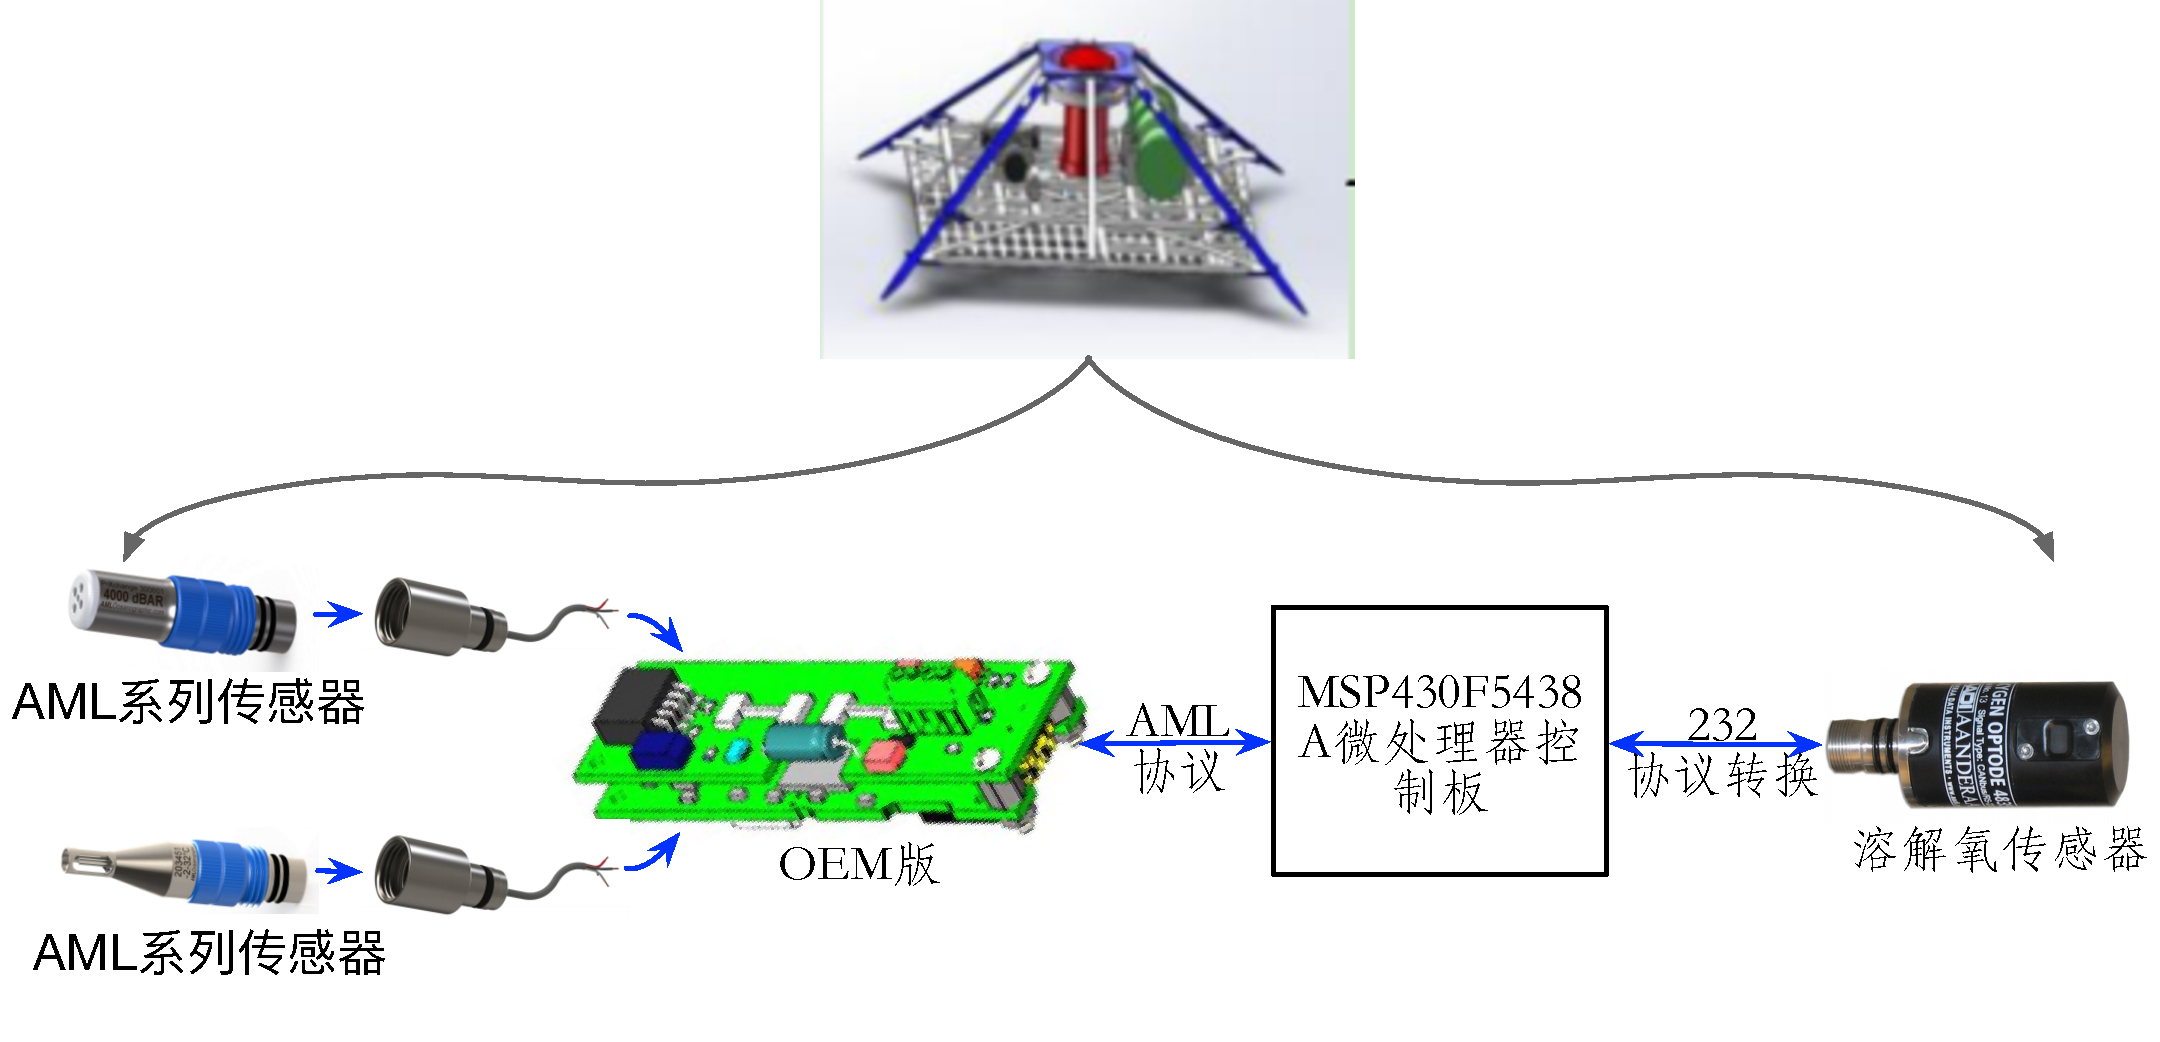
\includegraphics[width=1\textwidth]{fig/系统框图.pdf}
	\caption{海洋传感器集成系统整体架构图}
	\label{fig:系统框图}
\end{figure*}

传感器单元主要包括AML系列传感器和其他类型海洋传感器。AML系列传感器由于通信协议和接口都是一致的,通常它们可以互相替换,这些传感器通过OEM板与微处理器单元进行连接。其他类型的海洋传感器,比如溶解氧传感器等,通常是通过RS232或485协议与微处理器单元进行通信。微处理器单元主要包括MSP430F5438A为核心的最小系统和外围电路,比如用于传感器通信的协议转化电路、用于数据保存的存储电路等。

\section{系统硬件平台设计}
低功耗海洋传感器集成系统的硬件设计进行了多种海洋传感器的集成~\cite{2015cd},从而实现了对海洋生态环境数据的高效管理和采集。同时,还介绍了多个海洋传感器的特点和控制方法。作为一套较为完善且具有通用型的海洋传感器集成系统,后期还可能进行拓展集成。

不同的器件之间会存在供电电压的差异,使用相应供电电压的DC/DC转换器来解决电源供应问题,同时考虑到DC/DC电压转换模块的功率要求,以满足实际电路模块中的负载问题。

在系统设计中采用单处理器集中控制集成传感器,通过给传感器下达指令,完成数据采集等任务。考虑到系统的稳定性、可靠性以及后期的可拓展性,在数据通信模块中实现通信协议之间的转换,根据传感器数量对串口进行了相应的拓展。采用MSP430F5438A作为控制核心,它的作用至关重要,有超低的功耗和有良好的性能,同时拥有众多的接口资源。其中对于微处理器部分的设计框图如图~\ref{fig:微处理器}所示,传感器可以根据实际情况进行挂载或更换。
\begin{figure*}[ht]
    \centering
	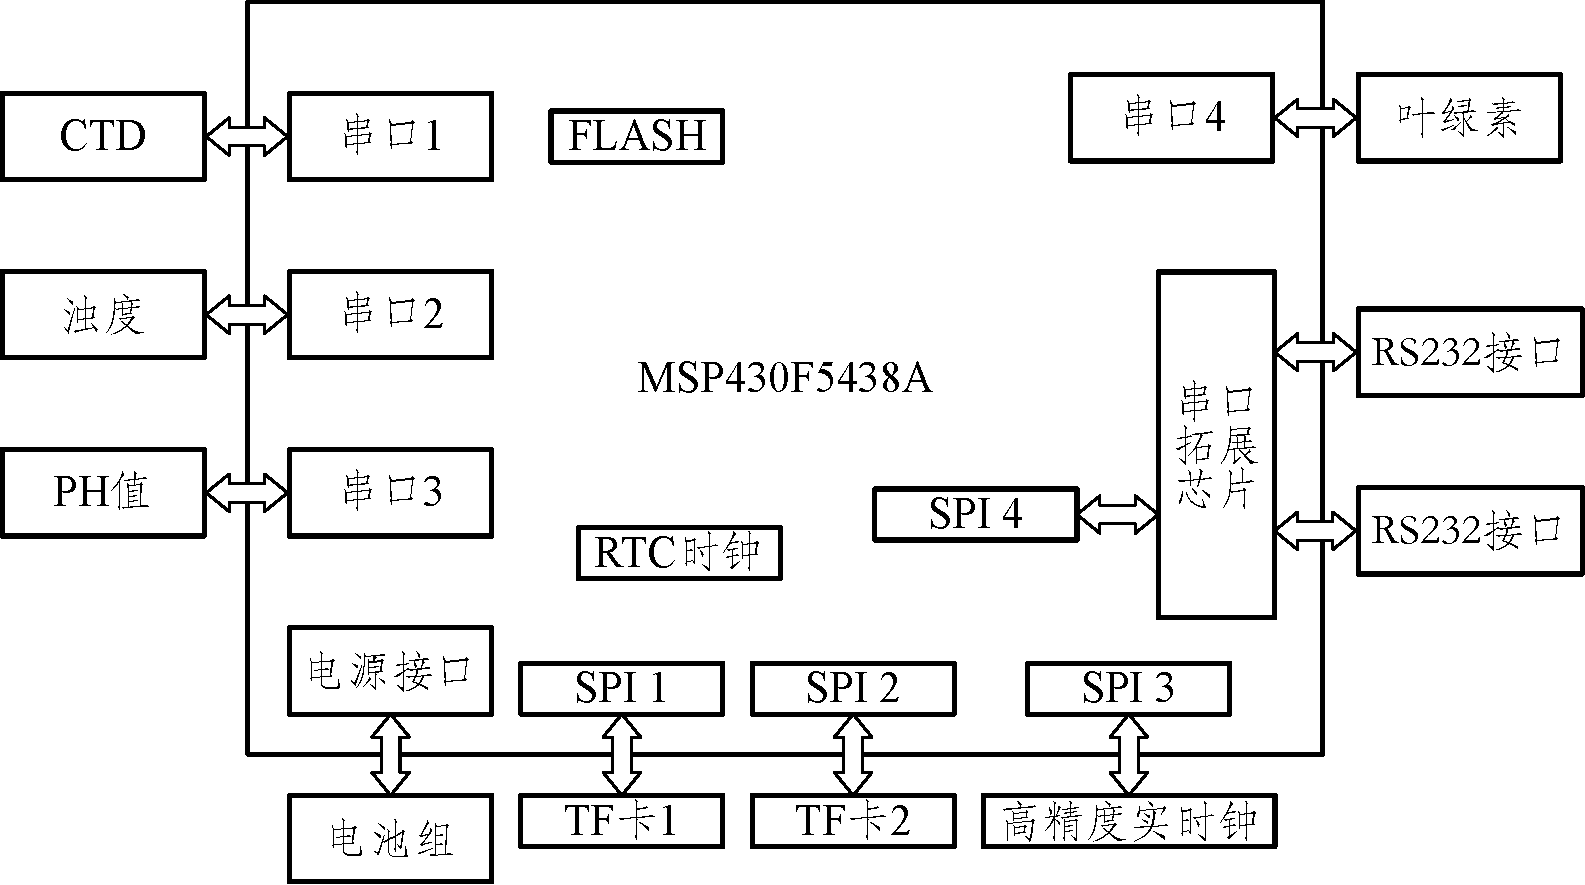
\includegraphics[width=1\textwidth]{fig/微处理器部分设计框图.pdf}
	\caption{微处理器部分设计框图}
	\label{fig:微处理器}
\end{figure*}

\section{系统软件平台设计}
低功耗海洋传感器集成系统的软件设计是整个系统设计环节的重要部分,只有高效、可靠的软件设计配合安全、可靠的硬件平台才能保证整个系统的稳定性。软件设计上实现传感器数据采集、数据存储、数据处理、数据回收等一系列操作,并在系统性能、微处理器资源配置、外设模块调度和软件逻辑框架上做大量研究,以保证系统以最低的功耗、最高的效率完成指定任务。软件平台分模块进行程序设计,通过系统管理与配置模块和数据采集与通信模块,分别实现与管理人员、海洋传感器之间的信息交互。能源管理与控制模块的软件设计实现了电源的有效控制,数据存储和回收模块对海洋生态数据进行有效的保存和处理。
\section{海洋传感器介绍}
在海洋观测与监测领域,海洋传感器被广泛应用于测量各种海洋环境因素,如温度、压力、深度等。电导率/盐度和其他基本物理参数海洋因素,对海洋资源的科学研究和开发具有重要意义。本文中海洋传感器需采集温度、深度、盐度、叶绿素、溶解氧、PH值、浊度、流速等海洋环境要素。

\subsection{AML多参数水质测量仪}
多参数水质测量仪可定点测量海洋各种生态环境要素,通过安装多个传感器探头即可采集不同的海洋要素。加拿大AML公司的AML Micro$\cdot$X传感器是一项重大进步在海洋仪器中。X代表是一个系列的海洋传感器,可依据现场状况和需要采集的海洋生态环境要素选择传感器负载。可交换和可互换的传感器极大地改善了海洋仪器多方面功能。在几秒钟内无需工具的情况下,即可在海上更改传感器的类型。例如,CTD可以通过更换传感器头将其更改为叶绿素分析器。为了优化传感器数据的分辨率和准确率,可以将传感器配置为可更改测量范围。

Micro$\cdot$X可以通过RS232或RS485串行连接进行通信。与传感器建立通信必须要使用正确的通信端口和设置。通信设置为8个数据位,1个停止位,无奇偶校验,无流量控制以及通信双方需同步波特率。波特率600、1200、2400、4800、9600、19200、或38400皆可以使用。当外部通信设备与传感器建立连接通信链路后就可以向传感器发送命令来完成状态显示、数据采集设置、数据检索和诊断测试工作。常用命令如下:

\begin{lstlisting}
SCAN:测量并输出一次数据扫描。
MONITOR:以设定的采样率进行扫描。
VERSION:显示仪器标识头。
DISPLAY OPTIONS:显示仪器状态和用户设置。
DISPLAY SAMPLE RATE:设置波特率。
\end{lstlisting}

Micro$\cdot$X传感器主要参数指标如表~\ref{tab:MicroX}所示。
\begin{table*}[h]
  \centering\small
  \caption{Micro$\cdot$X传感器参数表}
  \label{tab:MicroX}
\begin{tabular}{|c|c|c|}
\hline
\multirow{9}{*}{\bf 传感器测量范围和精度}      & 温度       & 范围: -5-45$^{\circ}$C  ,精度:  $\pm$ 0.003$^{\circ}$C          \\ \cline{2-3} 
                                           & 压力       & 范围: 
 50-6000dBar , 精度: $\pm$ 0.3\%FS                 \\ \cline{2-3} 
                                           & 盐度       & 范围:
0-42psu, 精度:$\pm$ 0.003psu              \\ \cline{2-3} 
                                           & 叶绿素      & 范围:
0-250ug/l,精度:   $\pm$ 0.2\%FS            \\ \cline{2-3} 
                                           & 浊度       & 范围 :
0-3000NTU,精度:   $\pm$ 0.5\%NTU         \\ \cline{2-3} 
                                           & PH       & 范围 :
0-14[PH],精度:$\pm$ 0.01[PH]             \\ \cline{2-3} 
                                           & 溶解氧      & 范围:
0-25mg/l,精度:$\pm$ 0.01mg/l               \\ \cline{2-3} 
                                           & 声速       & 范围 :
1375-1625m/s,精度:$\pm$ 0.006m/s           \\ \cline{2-3} 
                                           & 电导率      & 范围:
0-90mS/cm,精度:$\pm$0.003mS/cm            \\ \hline
\multicolumn{2}{|c|}{采样间隔}                  & 10min(设定)                         \\ \hline
\multicolumn{2}{|c|}{通信协议}                  & \multicolumn{1}{c|}{RS232/RS485}       \\ \hline
\end{tabular}
\end{table*}


\subsection{声学波浪流速剖面仪}
声学波浪流速剖面仪主要是用来测量波浪、流速剖面、方向波谱等海洋数据的传感器,简称AWAC,是一种适应性强且工作稳定的海洋监控设备。本文所讲的AWAC是基于挪威Nortek公司的产品来进行描述的~\cite{foteinis2017comparative},其工作原理主要依据多普勒效应,即在水中发送出一个短脉冲声波,在水中遇到障碍物时将会产生回音和频率的变化,据此数据对比用来测量水流的速度,同时还可以利用该传感器测量多种波浪数据~\cite{2016xcc}。

AWAC不仅可以实现使用内置电池和存储器的自容测量,还可以实现系统的在线观测。AWAC一般需要相应的挂载平台,一方面用于固定设备,另一方面可以减少外界对设备的损伤,为了防止设备生锈腐蚀,AWAC使用全塑料和钛合金材料制作外壳,使用钛合金材料不仅可以增大设备的看腐蚀性,还可以增大设备的耐压性。

\begin{table*}[htb]
  \centering\small
  \caption{AWAC技术指标和命令}
  \label{tab:AWAC}
\begin{tabular}{|c|c|c|}
\hline
\multicolumn{2}{|c|}{\bf 技术参数}                  &{\bf 性能指标 }                        \\ \hline
\multicolumn{2}{|l|}{工作频率}                  & \multicolumn{1}{l|}{10min流速剖面,1h波浪}                \\ \hline
\multicolumn{2}{|l|}{声学频率}                  & \multicolumn{1}{l|}{1MHz/600kHz/400kHz}                \\ \hline
\multicolumn{2}{|l|}{流速范围}                  & \multicolumn{1}{l|}{水平方向$\pm$10 m/s,光束方向$\pm$5 m/s}                         \\ \hline
\multicolumn{2}{|l|}{剖面范围}                  & \multicolumn{1}{l|}{30-40m}                     \\ \hline
\multicolumn{2}{|l|}{深度单元}                  & \multicolumn{1}{l|}{典型20-40层,最大128层}                       \\ \hline
\multicolumn{2}{|l|}{测量精度}                  & \multicolumn{1}{l|}{测量值的1\%或$\pm$0.5cm/s}                        \\ \hline
\multicolumn{2}{|c|}{\multirow{2}{*}{常用命令}} & \multicolumn{1}{l|}{Break-是仪器中断再重新启动}     \\ \cline{3-3} 
\multicolumn{2}{|l|}{}                          & \multicolumn{1}{l|}{ST-采样命令,串口输出数据} \\ \hline
\end{tabular}
\end{table*}

AWAC 有多种数据格式,如信息设置、传感器数据、流速数据、波浪特征参 数数据、波能量密度谱、波带特征参数、波浪傅里叶系数波谱~\cite{2014wjs}。在完成设备的基本设置后便可执行数据采集的工作,其相关技术参数如表格~\ref{tab:AWAC}所示。

\subsection{浊度传感器}
浊度传感器主要用来检测海水中悬浮物和胶状体对光线透过时所产生的阻碍程度,表征水样的光学性质,将依据悬浮物在水中存在漫反射等特性使用浊度传感器来检测水体的浑浊程度~\cite{2015wj}。主要是把水样的浊度转换为光电信号来进行检测,进而计算得出浊度值,具体可分为透射法、散射法等。

在本文中所使用的浊度仪器为美国Wetlabs公司所生产ECO-NTU浊度计,其表面采用具有自清洁功能的纳米防污材料,能够在海水环境中工作数月。并且具有耐腐蚀强、尺寸小、受光线影响小等优点,能够应用于海洋监测。相关技术参数如表格~\ref{tab:ECO-NTU}所示。

\begin{table}[htb]
  \centering\small
  \caption{ECO-NTU技术指标和命令}
  \label{tab:ECO-NTU}
\begin{tabular}{|c|c|c|}
\hline
\multicolumn{2}{|c|}{\bf 技术参数}                  & {\bf 性能指标}                         \\ \hline
\multicolumn{2}{|l|}{工作波长}                  & \multicolumn{1}{|c|}{700nm}                \\ \hline
\multicolumn{2}{|l|}{测量范围}                  & \multicolumn{1}{c|}{可选0-70NTU、0-200NTU、0-1000$\mu$g/L}                \\ \hline
\multicolumn{2}{|l|}{采样频率}                  & \multicolumn{1}{c|}{8Hz}                         \\ \hline
\multicolumn{2}{|c|}{波特率}                  & \multicolumn{1}{c|}{19200 baud}                     \\ \hline
\multicolumn{2}{|l|}{深度范围}                  & \multicolumn{1}{c|}{0-20/200$\mu$g/L}                       \\ \hline
\multicolumn{2}{|l|}{测量精度}                  & \multicolumn{1}{c|}{0.02$\mu$g/L}                        \\ \hline
\multicolumn{2}{|c|}{\multirow{2}{*}{常用命令}} & \multicolumn{1}{c|}{RUN-开始工作}     \\ \cline{3-3} 
\multicolumn{2}{|l|}{}                          & \multicolumn{1}{c|}{MVS-Bio刷开始/关闭} \\ \hline
\end{tabular}
\end{table}


\subsection{UV紫外灯}

在深海的环境进行长期的在线观测,海洋微生物的附着和海洋生物对设备的撞击都会影响到观测系统的正常运行。在过去十年中已经解决了对传感器的感测区域的保护的问题。比如,为了避免这些情况,往往会在观测系统中添加UV紫外灯。从而可以有效地防止生物污染。这将减少维护成本,提高收集数据的质量(减少与生物污损有关的干扰),并避免在环境中不必要地引入潜在有害的化学物质。
本系统采用AML公司的UV\_Xchange,它利用紫外线防止藻类及其他微生物生长在传感器的表面。UV光源光谱范围是200nm-450nm,以365nm为中心,光源可以有效防止微生物对水下设备的附着。UV紫外灯实物如图~\ref{fig:UV}所示。

\begin{figure*}[ht]
    \centering
	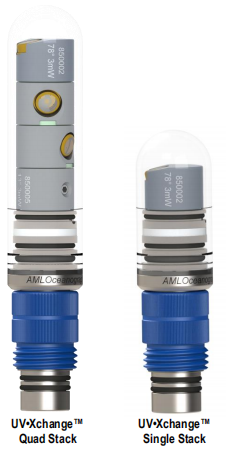
\includegraphics[width=0.3\textwidth]{fig/UV灯.png}
	\caption{UV紫外灯}
	\label{fig:UV}
\end{figure*}

\subsection{溶解氧传感器}
本系统采用安德拉公司的Oxygen Optode4835传感器。由于氧气参与了大多数水生生物和化学过程,所以氧气在海洋研究中可以作为一种示踪器。安德拉系列的溶解氧传感器具有长期稳定、受压力影响小、响应时间快等优点。设备可使用CAN总线或者RS-232总线与传感器进行连接,可以获取氧气的浓度、饱和度和温度。

Oxygen Optode 4835传感器的主要工作指令如下所示:
\begin{lstlisting}
"/"或";"(英文状态)指令      ******唤醒传感器
start指令                     *******传感器开始采集数据
stop指令                      ******传感器停止采集数据
measurement指令               ******传感器采集数据反馈
save指令                      ******保存传感器配置
\end{lstlisting}

\section{本章小结}
在本章节中对低功耗海洋传感器集成系统的整体架构进行了分体介绍,简略讲述了各部分的结构组成,并对其中每部分的独立功能进行了介绍,以论述海洋观测系统中各部分之间的组成关系以及工作关系,同时对传感器的性能指标做了简要概述。
\chapter{系统低功耗设计}
低功耗海洋传感器集成系统的设计目标就是长期于海底环境中对海洋水文数据定时采样。由于系统仅靠电池组维持电源供应,必须考虑系统的低功耗设计方案。系统采样时,微处理器处于活跃工作状态,并且控制电源给海洋传感器设备和电子器件进行电源供应;系统不采样时,微处理器处于休眠状态并且控制电源关断对各个器件的电源供应;如需再次激活系统,只需预先将微处理器唤醒,然后再恢复对系统的电源供应。系统低功耗设计具体实现主要从嵌入式微处理器选型和电源管理系统这两方面来入手。

\section{嵌入式微处理器选型}
在深海观测系统中,因受环境等因素的影响,嵌入式微处理器的选型应该考虑的因素有低功耗性、稳定性、计算能力、片内资源、开发环境、成本等。目前,市场上针对不同的应用场景开发出了多种微处理器芯片,可根据不同应用场景、不同功能需求选择不同系列不同资源的微处理器芯片,迄今为止电子市场比较主流的嵌入式微处理器芯片有以下几种:

C8051系列,应用最广泛的8位单片机,最早由Intel推出,内部集成AD、串口、SPI 接口,其I/O口使用较为简单且具备JTAG仿真功能。~\cite{2018wxp}。

MSP430系列,是TI公司推出的一种16位超低功耗的混合信号处理器,特点是在以超低的功耗保持较为强大的处理能力,其架构与多种低功耗模式配置使用,是延长便携式应用电池寿命的很好选择。在超低功耗方面,其可灵活控制时钟的运行以降低功耗,时钟关闭时其电流最低可降低到0.1uA~\cite{2008wx}。

Cortex系列,是ARM公司针对不同的应用环境推出的Cortex系列微处理器芯片,其中Cortex-M3 是一种基于ARM V7架构的最新ARM32位处理器内核~\cite{zhao2017design}。Cortex系列微处理器一般都有很丰富的外设资源,同时还兼备实时性能和优异计算能力的特点。 Cortex-M3的电源管理方案通过NVIC支持Sleep Now、Sleepon Exit、SLEEPDEEP 三种睡眠模式,使其能够以较低的能耗实现超丰富的功能~\cite{wx} 。

该系统的微处理器芯片选型主要参考以上三个系列,其中应用广泛的C8051系列虽然满足低功耗、廉价的条件,但是其可扩展性较差,计算能力方面也有不足,且自我保护的能力很差,满足不了该系统的稳定性原则,因此不适合本系统。低功耗海洋传感器集成系统需要携带相对较少的电池能源以减少水密舱的体积增加存活率提高整个系统的生存周期,所以系统的微处理器芯片选型时,低功耗的优先级略大于计算能力和片内资源。因此系统选用了处理能力略低于Cortex-M系列但低功耗性能突出的MSP430系列中的MSP430F5438A微处理器。

\section{电源管理}
关闭系统的电源是最为节省能耗的措施。系统外部电路设备的电源可通过微处理器来控制关闭,就可以降低电池组的能耗。在很多MSP430的应用中,电子仪器都是在有限的时间内保持运行。在电子仪器非工作的时间内保持电源持续的供应,这一部分造成的能源浪费是完全可以避免。通过提高能源利用效率的手段来降低功耗。

在低功耗海洋传感器集成系统应用中,电源管理部分是整个系统节省能源、实现长期稳定工作的关键。MSP430F5438A微处理器可通过设置寄存器来控制CPU进入到不同的工作模式当中,休眠状态比活跃状态节省很大的能源消耗。同时可控制的DC/DC模块通过微处理器的IO口进行设置,IO口的输出信号连接DC/DC模块的Ctrl引脚,这样即可通过IO口输出高电平或者低电平来控制DC/DC模块的开启或关闭~\cite{2013xyd}。

整个系统的能源消耗由MSP430芯片和其他模块电路能源消耗构成。微控制器芯片的内部集成大量的模拟外设,这些外设的工作状态对于整个系统的能源消耗有很大的影响~\cite{2005xy}。内部的部件可分为模拟部件和数字器件,工作频率的变化对数字部件有很大的变化,而模拟部件的功耗在不同频率下几乎没有变化。模拟部件和数字部件的能源消耗之和相当于整个芯片的总功耗。
\begin{equation}
\begin{split}
\mathcal{P} = CV^2f
\end{split}
\label{eq:example}
\end{equation}   

本系统一直在关注低功耗的要求,但是低功耗到底如何来定性的衡量。由公式\ref{eq:example}可知,功耗由三个要素决定,分别是C(负载电容)、V(供电电压)、f(系统的工作频率)~\cite{2007hsj}。从中可以看出电源电压对功耗的影响是最为关键的,工作频率、负载电容的决定性则次之。而由于在系统设计当中,负载电容往往是不可控制的,不会在电路设计和器件选型中有意的去降低负载电容。在不影响整个系统性能的前提下,为了实现系统低功耗的要求,应该着力于研究如何降低供电的电压、时钟进行各种工作模式的切换以求降低时钟频率对功耗的影响。

\subsection{电源电压管理}
电源电压管理主要从两个方面来降低整个系统电源电压以实现降低整个系统功耗的目的。一方面设计采用的MSP430F5438A具有低电源电压范围(3.6V到低至1.8V);另外一方面,系统中可以对DC/DC模块进行程序控制,在给到相应DC/DC模块Ctrl引脚的信号为高电位时,即开启了此处的电源供应,这部分的负载才会消耗电源电压,否则就会一直处于关闭的状态,节省了能源消耗。

整个系统的电源消耗由微处理器芯片内部集成的很多模拟外设和其它模块电路能源消耗组成。因此芯片内外的外设工作情况对整个系统的能源消耗起到决定性的影响。 

\subsection{时钟切换控制}
系统工作频率方面,主要是通过对微处理器件进行合理的时钟切换来降低整个系统的功耗。在上一章的硬件平台设计中,详细的描述了MSP430的基本时钟系统,这里就不再赘述。作为一款超低功耗的微控制器,MSP430本身的多种工作模式就为应用者进行低功耗设计提供了极大的便利。MSP430系列微处理器具有如表~\ref{tab:CTC}所示的不同工作模式。

%\newcommand{\tabincell}[2]{\begin{tabular}{@{}#1@{}}#2\end{tabular}}  
%表格自动换行
\begin{table*}[ht]
\caption{工作模式}
\label{tab:CTC}
\centering
    \begin{tabular}{|c|c|c|c|c|c|}
        \toprule
        {\bf SCG1} & {\bf SCG0} & {\bf OSCOFF}& {\bf CPUFF} & {\bf 模式}&{\bf CPU和时钟状态}  \\      
%\bf表示字体加粗
        \hline
        0  & 0  & 0 & 0& 活动模式& \tabincell{c}{CPU、MCLK活动模式。ACLK活动。\\SMCLK选择性活动 (SMCLKOFF=0)。} \\
%需要分行的单元格的语句用\tabincell{c}{所填写第一行内容\\第二行内容···},可以根据需要换行,也不限定换多少行。
        \hline
      0  & 0  & 0 & 1& LPM0& \tabincell{c}{CPU、MCLK禁止。ACLK活动,\\SMCLK有选择的活动(SMCLKOFF=0)} \\
        \hline
      0  & 0  & 0 & 1& LPM1& \tabincell{c}{CPU、MCLK禁止。ACLK活动,\\SMCLK有选择的活动(SMCLKOFF=0)} \\
        \hline
      0  & 1  & 0 & 1& LPM2& \tabincell{c}{CPU、MCLK禁止。ACLK活动,\\SMCLK有选择的活动(SMCLKOFF=0)} \\
     \hline
      0  & 0  & 0 & 1& LPM3& \tabincell{c}{CPU、MCLK禁止。ACLK活动,\\SMCLK禁止} \\
     \hline
      0  & 0  & 0 & 1& LPM4& \tabincell{c}{CPU和所有的时钟都禁止} \\
        \bottomrule
    \end{tabular}
\end{table*}

激活模式(AM)是所有的时钟激活;待机模式(LPM3)下带有晶振的实时时钟(RTC),看门狗和电源监视器工作,完全RAM保持,快速唤醒;关闭模式(LPM4)下完全RAM保持、电源监视器工作、快速唤醒。不同工作模式下供电电流的差别是极大的~\cite{2005xy},不同工作模式下典型的电流值如表~\ref{tab:dl}所示。

\begin{table}[ht]
\caption{各种工作模式的典型供电电流值($\mu$A)}
\label{tab:dl}
\centering
    \begin{tabular}{|c|c|c|}
        \hline
        \diagbox{\bf$\mu$A}{\bf 电压} & 2.2V & 3.0V \\   
        %斜线命令语句
        \hline
        I(AM) &280 &420 \\
         \hline
        I(LPM0) &32 &55 \\
         \hline
        I(LPM2) &11 &17 \\
         \hline
        I(LPM3) &0.9 &1.6 \\
         \hline
        I(LPM4) &0.1 &0.1 \\
         \hline
    \end{tabular}
\end{table}

工作模式的选择主要考虑超低功耗、强大的数据处理能力和外围模块功耗最小这三个方面的要求。MSP430F5438A具有五种低功耗模式(LPM0-LPM4)~\cite{2005wdy}和一种活动模式,低功耗模式LPM0-LPM4可以通过设置状态寄存器来实现。针对不同需求的应用场合,设计中应合理选择工作模式和时钟频率。比如在ADC周期性采样、串行通信等应用场合之下,需要在工作时间内保持主时钟频率。本系统中一般处于LPM3模式下,之所以选择LPM3模式是考虑到LPM4模式下CPU及所有的时钟(ACK)都禁止,但是系统要求软时钟在低功耗的模式下仍然可以使用且可中断唤醒CPU。任何使能的中断事件都可以把MSP430从低功耗模式(LPM0到LPM4)中唤醒。程序控制单片机在指定的时刻通过定时器中断进入活动模式。

\section{本章小结}
本章主要阐述了低功耗海洋传感器集成系统的低功耗设计,首先概述了低功耗设计的总体方案,然后对器件选型方面如何考虑低功耗要求进行分析,最后着重于描述系统电源管理,分别从降低供电电压和时钟切换控制方面来降低系统的能源消耗。







\chapter{系统硬件平台设计}
低功耗海洋传感器集成系统将集成多种海洋传感器,主要目的是针对传感器进行有效管理。系统在低功耗的指标下可通过对传感器下达控制和工作指令从而获取海洋水文数据的采集,数据可进行本地存储,也可通过预留接口对传感器采样数据进行回收。系统硬件平台    主要由传感器连接控制模块和微处理器模块两大部分组成。其电子电路的设计上主要受系统稳定性、系统功耗和电路板PCB大小限制,在保证功能稳定的前提下,应该优先选择具备功耗控制功能和较小封装的外设芯片以确保系统的电子电路在规定的有限舱体内长时间稳定工作。整个硬件设计在稳定性和低功耗性方面做大量研究,实现安全可靠的硬件观测平台,为系统的稳定运行提供保障。
\section{传感器连接控制模块}
传感器连接控制模块主要负责各海洋传感器的管理工作及状态监控等,具体包括传感器电源控制、数据通信协议转换等,电源控制部分设计关键在于需要根据不同传感器负载选用不同型号的DC/DC电压转换模块,经由微处理器来控制其开关;传感器数据通信部分主要使用了串行设备通信协议,根据本文中的传感器数据传输协议~\cite{2017jy}和接口类型,在该模块中,AML系列海洋传感器都统一使用AML专用的传输协议,其他类型传感器主要采用了RS232或RS485接口进行通信,传感器模块给微处理器传输状态信息和采样数据,同时微处理器也可以经过该方式给传感器下达传感器配置、采样、查询等命令。
\subsection{电源供应与分配部分}
由于整个系统各个模块所需求的电压不同,所以对接入电压需进行合理的转换分配,以满足各模块的正常工作。在电子电路中设计了电压转换电路可以避免使用多个电压源造成电池能源和舱体空间的浪费。为了达到低功耗的要求,给海洋传感器供电时应考虑可控性。因而采用控制式的DC/DC电压转化模块,用于实现对海洋传感器的上电与断电。

对于DC/DC模块的选用,主要依据于各个模块、器件所需工作电压和工作功率的要求。为了保证各电子器件能够工作,需要将接入电压~\cite{yzx}转换成各器件所需的工作电压,比如9V、5V或3.3V等。低功耗海洋传感器集成系统的能源都是来自于携带的电池组,电池组由七节锂电池串联而成,每节锂电池的电压范围是:3.8\-4.2V。由于锂电池随着电池容量的变化,电压也会出现变化,这也要求DC/DC模块具备宽输入电压。系统的处理器MSP430F5438A和其他模块芯片所需要的正常工作电压是3.3v。因此需要将接入电压转化为3.3V,主要通过相对应的DC/DC电压转化模块来完成,相关电路原理图如图~\ref{fig:DC3.3V}所示。

\begin{figure*}[ht]
    \centering
	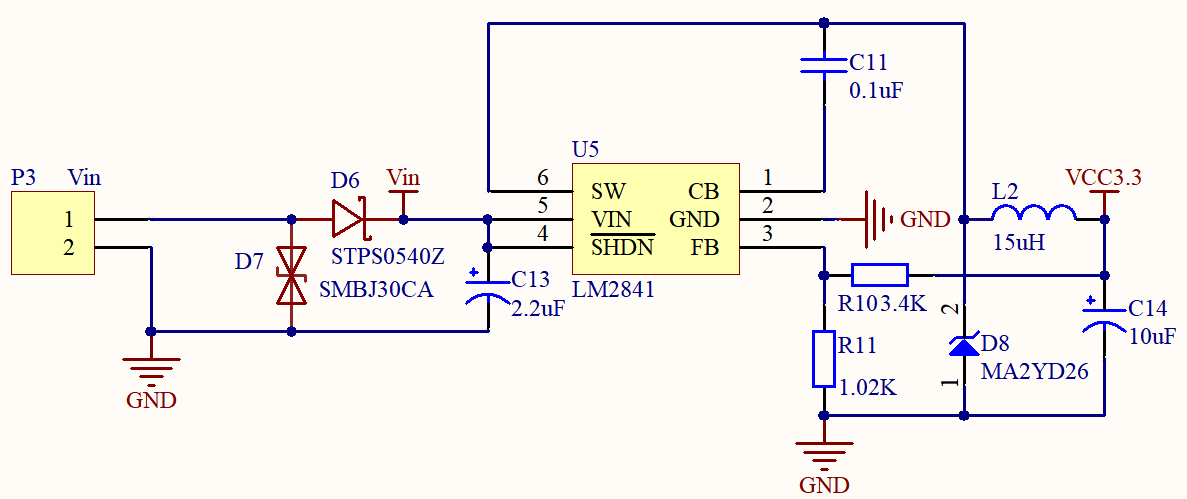
\includegraphics[width=0.8\textwidth]{fig/DC_3.3.png}
	\caption{转DC3.3V电路原理图}
	\label{fig:DC3.3V}
\end{figure*}
                                                
DC/DC电压转化模块选用了TI公司的LM2841,这款DC/DC降压调节器的输入电压范围从4.5V到42V,输出电流300mA,适合于广泛的应用。最大效率可达85\%,同时具有软启动的功能可实现控制上电断电(SHND引脚拉到GND以禁用设备,拉高以启动设备)。输出电压可设置,通过公式\ref{eq:功率}可计算输出电压,根据实际需要的电压,来设置R10和R11的电阻比。
\begin{equation}
\begin{split}
\mathcal{V}_{OUT} = 0.765 V (1 + (R10/ R11))
\end{split}
\label{eq:功率}
\end{equation}   

通常,R11被赋予100Ω到10kΩ的起始值。

\subsection{传感器电源管理部分}
对于海洋传感器的供电问题,将使用DC/DC电源模块将接入的电源电压转换为海洋传感器正常工作需要的电压(9V)为其供电。海洋传感器的电源管理使用带有Ctrl端可控的隔离稳压电源模块,从MSP430控制芯片下达控制指令,对传感器进行上电和断电的操作。将接入电压转9V的具体电路实现如图~\ref{fig:DC9V}所示。

\begin{figure*}[ht]
    \centering
	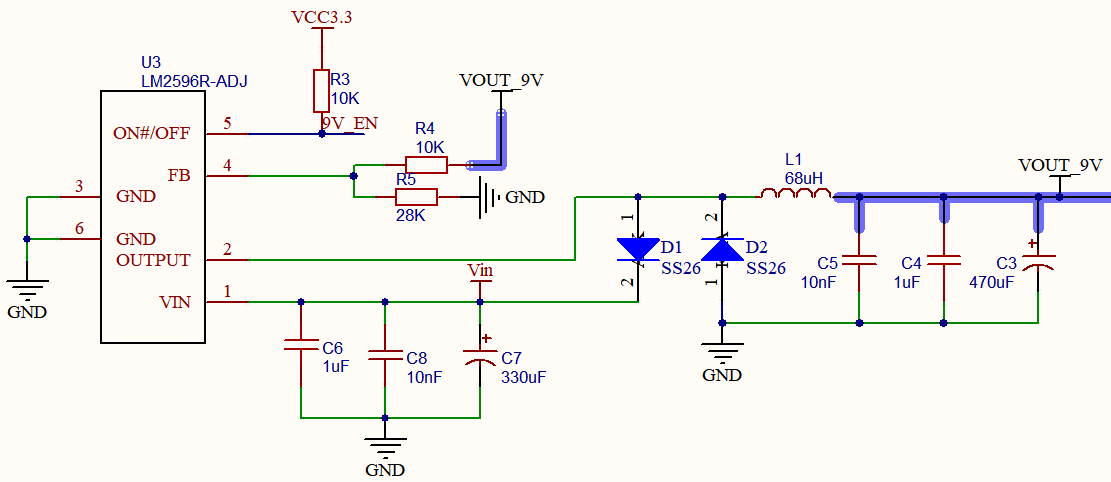
\includegraphics[width=0.8\textwidth]{fig/DC_9V.png}
	\caption{转DC9V电路原理图}
	\label{fig:DC9V}
\end{figure*}

电子电路设计中使用了LM2596降压DCDC芯片,其具有程序可控、输出效率高、宽输入电压范围、输出过压保护、过流保护以及短路保护的特点。高效率、大电流、低纹波的特点满足设计要求。可实现将DC12V输入转9V,同时较大的输出电流,也能够满足多个传感器负载。

\subsection{传感器数据通信部分}
该部分实现的功能主要是将不同传感器的通信方式转换为能够直接与微控制器相连的电平信号,本系统为微处理与海洋传感器连接提供了两种数据通信协议,其一为常用的RS232通信协议标准(一种点对点的数据传输方式),使用较为简单,只需将TX、RX、GND进行连接后即可完成相关的通信流程;其二是与AML系统海洋传感器连接的特定协议。

\subsubsection{RS232协议转换部分}
微处理器与海洋海洋传感器通信接口采用RS232标准。RS232协议支持全双工传输数据,其通信标准可以以九针接口定义,也可以使用三针接口定义~\cite{2020xxw}。本设计使用三针的接口定义,只需要使用TX、RX、GND三个引脚,利用MAX323SE实现TTL电平到RS232电平的转换,该芯片具有较好的低功耗性能,供电范围为3V-5.5V。具体电路实现如图~\ref{fig:RS232}所示。

\begin{figure*}[ht]
    \centering
	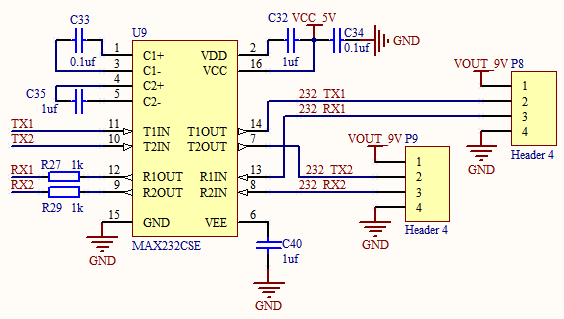
\includegraphics[width=0.8\textwidth]{fig/RS232.png}
	\caption{电平转换电路}
	\label{fig:RS232}
\end{figure*}

对于不同接口的海洋传感器,如RS422或RS485通信接口,可以选用相应型号的转换芯片来支持对应的接口。

\subsubsection{AML传感器连接部分}
AML\uline{ }Xchange系列传感器需要特定的电气协议和数据接口与设备连接,所有的AML智能传感器共享相同的电源。AML\_ Xchange系列传感器通过特定的传感器接口与OEM板连接,OEM板再与微处理器之间直接进行通信(TTL电平协议通信)。OEM板连接图如图~\ref{fig:OEM板连接图}所示:

\begin{figure*}[ht]
    \centering
	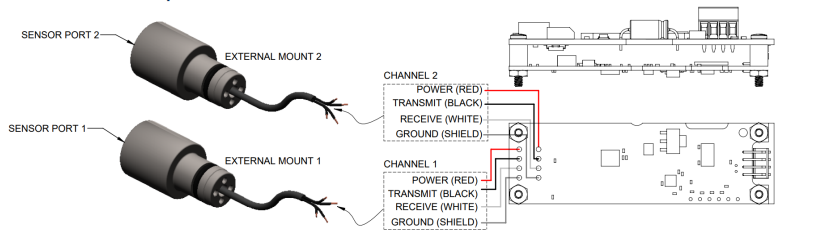
\includegraphics[width=\textwidth]{fig/OEM板连接图.png}
	\caption{OEM板连接图}
	\label{fig:OEM板连接图}
\end{figure*}

每块OEM板上有两个传感器通道,通道有电源、地、接收、发送四个引脚。OEM板接上传感器接口后,AML\_Xchange系列传感器插头旋拧进接口就形成了完整的连接。AML\_Xchange系列传感器插头实物如图~\ref{fig:AMLXchange}所示。

\begin{figure*}[ht]
    \centering
	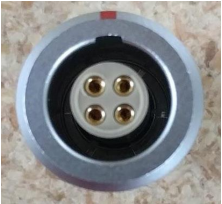
\includegraphics[width=0.3\textwidth]{fig/AML_Xchange.png}
	\caption{AML\uline{ }Xchange系列传感器插头}
	\label{fig:AMLXchange}
\end{figure*}

由于不同类型传感器共享相同的电源,且接口是一致的。如需更换传感器的类型,将其从OEM板接口拧出,更换上相应的传感器即可。

\section{微处理器模块}
微处理器模块是整个平台最为核心的部分,是系统完成各项功能的控制中心,承载着水下所有数据采集任务。该模块主要由MSP430F5438A控制芯片构成的最小系统、串口拓展电路、数据存储电路以及数据回收接口电路组成。
\subsection{最小系统}
最小系统主要由MSP430F5438A微处理器芯片、时钟电路、复位电路和下载电路组成。TI MSP系列超低功耗控制器种类繁多,可针对不同的应用需求进行选择。该微处理器具有优越的低功耗性能,当系统不需要进行工作任务时可根据最低电源消耗、最快速启动时间和可用唤醒源选择进入某一种低功耗模式。在系统处于非任务状态下配置成LPM3低功耗模式,该模式下功耗典型值小于2uA。MSP430具体架构如图~\ref{fig:MSP430架构}所示:

\begin{figure*}[ht]
    \centering
	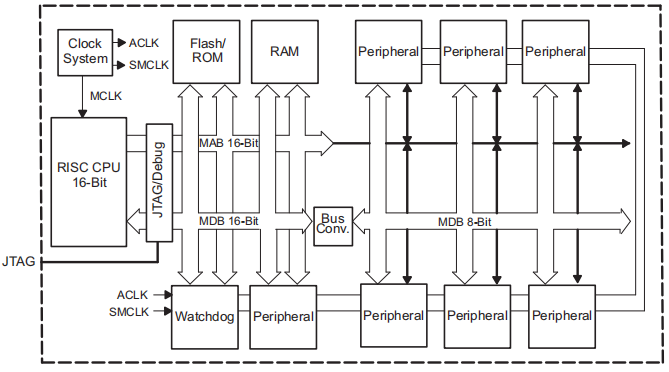
\includegraphics[width=0.8\textwidth]{fig/MSP430架构.png}
	\caption{MSP430架构}
	\label{fig:MSP430架构}
\end{figure*}

\subsubsection{微处理器时钟系统} 
从最基本的时钟系统出发,能够直观的理解MSP430F5438A这款微处理器芯片。这里对时钟系统进行简要的介绍。标准时钟系统(Unified Clock System(UCS))可以为芯片提供各种所需的时钟信号。MSP430F5438A的UCS模块由主系统时钟(MCLK)、子系统时钟(SMCLK)、辅助时钟(ACLK)以及专用时钟(MODCLK)这四个时钟系统组成~\cite{sxf}。

本系统的外部高速晶体振荡电路采用16MHZ的高速晶振,晶振连接到XT2IN和XT2OUT。但是上电后,XT2会一直保持静止状态,直到通过PSEL设置成XT2模式,PSEL置位,XT2IN和XT2OUT将配置成XT2模式。如果与XT2IN对应的PSEL位清零,XT2IN和XT2OUT均会被配置为普通的IO口模式,此时XT2的功能是禁止的。外部高速时钟源电路如图~\ref{fig:外部时钟源电路}所示:

\begin{figure*}[ht]
    \centering
	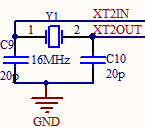
\includegraphics[width=0.5\textwidth]{fig/外部时钟源电路.png}
	\caption{外部高速时钟源电路}
	\label{fig:外部时钟源电路}
\end{figure*} 

\subsubsection{下载电路} 
进行软件调试时,通常会直接烧写程序或者在线仿真,仿真和烧写有几种方式可供选择。最常见的是JTAG方式,可以访问到MSP430所有资源。JTAG既可以对MSP430进行仿真也可以编程,需要使用的主要连线有TMS、TCK、TDI、TDO。图~\ref{fig:JTAG接口定义图}是JTAG的接口定义图。

\begin{figure*}[ht]
    \centering
	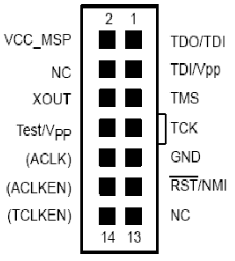
\includegraphics[width=0.4\textwidth]{fig/JTAG接口定义图.png}
	\caption{JTAG接口定义图}
	\label{fig:JTAG接口定义图}
\end{figure*}


SBW(SPY-BI-WIRE)又简称为两线制JTAG,只需要SBWTCK、SBWTDIO这两根线路。SBW既可以留有更多的IO资源,也可以让设计的PCB板更加小型化。电子电路设计中,在满足性能指标的情况下,尽可能选择简化设计的方法,对于本系统的微型化设计的目标具有重要的意义。下载电路如图~\ref{fig:下载电路}所示:

\begin{figure*}[ht]
    \centering
	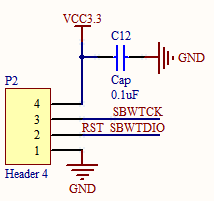
\includegraphics[width=0.5\textwidth]{fig/下载电路.png}
	\caption{下载电路}
	\label{fig:下载电路}
\end{figure*}

\subsubsection{外部复位电路}
嵌入式微处理器MSP430F5438A的内部复位信号在NRST引脚上,内部的脉冲发生器保证每一个复位源有20us的脉冲延时,当NRST引脚被拉低产生外部复位信号时。硬件原理图如图~\ref{fig:外部复位电路}所示。
\begin{figure*}[ht]
    \centering
	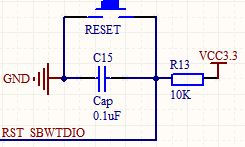
\includegraphics[width=0.5\textwidth]{fig/外部复位电路.png}
	\caption{外部复位电路}
	\label{fig:外部复位电路}
\end{figure*}

\subsubsection{实时钟电路}
本系统需要长期工作于深海环境之下,在甲板上设置好参数之后,从设备投放海底到回收期间,系统会自动化的采集海洋水文数据,相关的外部工作人员除非出现设备故障,否则不会有工作人员对系统设备进行干预。一方面在电源管理的部分,需要定时周期性的给电子设备和海洋传感器设备进行供电;另外一方面,在进行数据采集时,需要加上时间戳并且各种不同的海洋水文数据需要同步测得,这种数据采集才具备研究的价值和意义。高精度实时钟能够在系统参数配置的阶段接受到工作人员发送来的系统时间,从设定的系统时间开始计时。程序可以记录上一次数据采集的时间,并计算下一次数据采集的时间。

MSP430F5438A是自带实时钟模块(RTC)的,提供带日历、可编程闹钟和校准功能的时钟计数器。供电引脚VBAT脚采用混合供电的方式,由CR2110纽扣电池和3.3V电池同时供电,确保RTC的运行。RTC\_A模块是计数增加的时钟源可以是ACLK、SMCLK或者是分频之后的ACLK或者SMCLK。为了方便RTC\_A日历的操作,ACLK必须设置为32768Hz(通常情况)。由于时钟源不论是选择内部时钟,还有选择外部晶振产生的时钟都会产生比较大的时间误差。

低功耗海洋传感器集成系统是铺设在海底环境当中的,进行数据采集记录时间戳需要较为精准的时间。如果要外部的工作人员去进行时间校准的话成本会很大,所以对于实时钟的时间准确度和稳定性是有极高的要求的。本系统选用了极端精确的带有集成晶体和SRAM的SPI总线时钟芯片DS3234。为确保电路的稳定性和安全性同时提高CS和INT的高电平输出能力,分别在片选线和中断触发上接10k上拉电阻。具体的电路实现如图~\ref{fig:高精度实时钟电路}所示:

\begin{figure*}[ht]
    \centering
	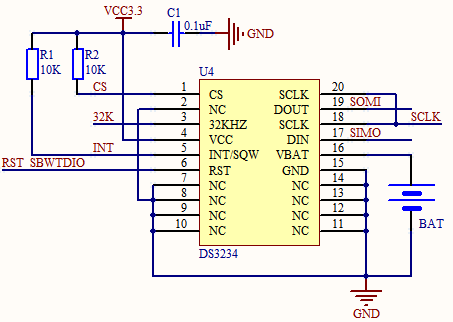
\includegraphics[width=0.6\textwidth]{fig/高精度实时钟模块电路.png}
	\caption{高精度实时钟电路}
	\label{fig:高精度实时钟电路}
\end{figure*}

DS3234具有低成本、高精度的优点。它可以提供一个稳定而精确的参考时钟,误差在每年2分钟之内。通过SPI总线的方式与MSP430微控制器进行通信。DS3234作为SPI串行总线的从设备,通过CS脚进行片选。DS3234数据传输方式具有很大的灵活性,支持单字节和多字节两种数据传输。在32K这个引脚上可以输出一个稳定32KHZ频率的时钟源给到MSP430微控制器。DS3234具备闹钟的功能,当系统时间与设定的闹钟时间达到一致时,在INT/SQW引脚上会产生一个中断信号给微处理器。

\subsection{串口拓展电路}
串口通信在计算机、工业控制、自动化等领域应用广泛,常见的串口通信协议有RS232、RS422、RS485等,都是各仪器设备通用的通信协议。RS232通信协议使用比较简单,通信速率较低,通信距离一般不超过25米,通常用于点对点的数据传输;RS422采用平衡方式传输,根据两条传输线之间的差分信号来判断逻辑状态,拥有比RS232更强的驱动能力~\cite{2020wqh}。RS485串口通信可实现2线半双工和4线全双工,传输距离可达1.2Km,现在多采用两线制方式,这种总线式拓扑结构可实现同时挂接32个以上设备,可实现一主多从的通信方式~\cite{2016cmy}。MSP430F5438A微处理器自身具有4个普通串口(UART)。

根据系统要求,海洋传感器需要普通串口四路(每路具有两个通道),还要有两路作为备用,所搭载的海洋传感器多为AML系列,其它的海洋传感器通信方式都为RS232串行通信,为了满足多种类型海洋传感器集成搭载的需求,因而对串口资源进行了拓展。

\begin{figure*}[ht]
    \centering
	\includegraphics[width=0.7\textwidth]{fig/wk2124.png}
	\caption{串口拓展电路}
	\label{fig:串口拓展电路}
\end{figure*}

本文所采用的拓展芯片为成都为开微电子公司的WK2124。WK2124采用的是SPI接口,有四个通道的UART。它是低功耗设计,可以配置为自动休眠、微秒级自动唤醒模式。主UART支持波特率自动适应,宽工作电压设计2.5V\-5V,各UART通道都有与之对应的寄存器和控制字,方便对各通道进行控制。

WK2124的主接口接到MSP430F5438A的SPI总线,需要MOSI、MISO、VCC和GND四根线进行连接即可,通过SPI总线协议转UART协议进行数据通信。需要注意的是,上电复位后,WK2124需要先写入OX55,其可以自动测得微处理器的波特率,并锁定主UART的波特率,之后WK2124和主机的通信就按照此波特率进行;如果需要更换其他的波特率,则需要对芯片进行硬件复位操作,然后在进行波特率测试和锁定。WK2124具体的电路实现如图~\ref{fig:串口拓展电路}所示:

WK2124采用+3.3V供电,RST是硬件复位引脚,低电平有效,复位期间及复位后,各子串口处于禁止收发状态,当子串口处于联网状态下,该特性使得该子串口所在的子节点在上电、复位期间不会对联网的其他子节点产生干扰。此外,各子串口也可以实现软件复位。RST\_SBWTDIO节点也可以接微处理器芯片的普通I/O引脚,用于通电期间的复位操作。

WK2124的中断输出引脚IRQ一般接微处理器的外部中断引脚。WK2124有两级中断:子串口中断和全局中断。全局中断寄存器GIFR用以判断中断类型,然后在相应的中断状态寄存器中可以读取到当前的中断源。此外,WK2124的每个子串口都有独立的中断系统,包括FIFO数据错误中断,发送FIFO触发点中断等。中断被使能以后,满足中断触发条件就会触发对应的中断。

\subsection{数据存储电路}
在低功耗海洋传感器集成系统中,可以把采集到的海洋水文数据存储于TF卡中。SD卡是一种便携的可移动存储设备,数据传输快、支持热插拔。TF卡,又称Micro SD卡,体积约是SD卡的1/4,和SD卡相比体积较小,适于小巧或空间有限的设备使用。

TF卡和SD卡的通信协议和编码地址都是一样的,通信协议为SPI总线~\cite{2015zjh}和SD总线,虽功能相同,但接口不同。TF卡的优势不言而喻,在实际开发和应用中,占据物理空间更小的TF卡会得到更广泛的使用。SPI总线相比SD总线虽有通信速率上的不足,但是也很明显的优势就是简化主机的设计。

在本系统中主机和TF卡之间选取了SPI总线进行数据通信。这是出于两个方面考虑的:MSP430F5438A微控制器的SD模式引脚被其它模块所占用,为了简化主机的设计和节省微处理器资源;SPI总线的数据通信速率是能够满足海洋传感器集成系统中数据采集的要求的。

TF卡存储电路实现原理图如图~\ref{fig:TF卡电路}所示:

\begin{figure*}[ht]
    \centering
	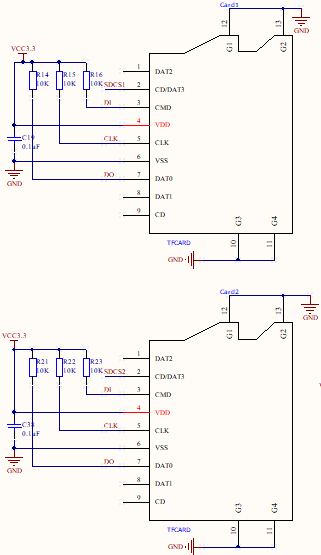
\includegraphics[width=0.5\textwidth]{fig/TF卡电路.png}
	\caption{数据存储电路}
	\label{fig:TF卡电路}
\end{figure*}

系统中采用TF卡的主要作用就是将海洋传感器数据存储于TF卡当中。此功能和USB挂载硬盘类似,但是用TF卡功耗比较小,所占物理空间也比硬盘小得多。虽然系统在海底环境需要长期进行采样,但是数据采集不是连续的。数据储存量要求并没有太高,用TF卡是能够满足储存采集数据要求的。
\subsection{数据回收电路}
低功耗海洋传感器集成系统中采集到的海洋水文数据,一方面可以通过本地存储保存在TF卡中,另一方面可以通过预留出接口把数据进行回收。本系统设计采用CH340E芯片将串口转成USB接口方便用来进行调试和回收采集数据。当设备从海洋环境当中打捞出来时,个人计算机只要接上USB线就能便捷的获取海洋传感器采集数据和整个系统的状态;系统出现故障时,维修人员将系统设备从海底打捞上来,接上USB接口也能及时进行系统调试,对于系统的现场维护具有重要意义。具体的USB接口电路实现如图~\ref{fig:USB接口模块原理图}所示。

\begin{figure*}[ht]
    \centering
	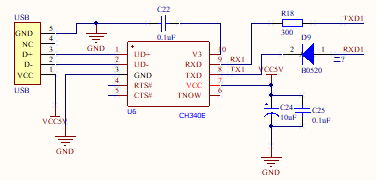
\includegraphics[width=0.7\textwidth]{fig/usb.png}
	\caption{USB接口电路原理图}
	\label{fig:USB接口模块原理图}
\end{figure*}

本模块选用串口转USB芯片CH340E,可实现串口转USB。CH340E芯片只有10个引脚,简化设计的同时还节省了设备的空间。从原理图~\ref{fig:USB接口模块原理图}中可以看出MSP430F5438A的串口一升级成USB总线。计算机通过USB总线与微处理器控制板进行连接,方便进行串口测试,另外可使用USB总线直接进行串口下载程序。所以USB接口模块很大程度上优化了系统的测试和使用便捷性。

\section{可靠性和冗余设计}
系统中采集到的海洋水文数据进行储存时,主机对TF卡可能既要进行读操作又要进行写操作。但是从以往实际应用TF卡存储的经验中发现:在进行读写操作时,读写可能不稳定从而导致数据会出现丢失的情况。从原理图~\ref{fig:TF卡电路}中可以看到,TF卡存储模块采用了冗余设计。在对TF卡进行写时,进行两次写操作,数据既要写入到TF卡一当中,又要写入到TF卡二当中。其中一块存储卡写发生故障或者数据丢失时,仍能够保证数据安全的本地保存。这样做的好处是,提高系统的可靠性,通过备份的手段,保证了数据读写的稳定性,增强系统的鲁棒性。


\section{本章小结}
本章阐述了低功耗海洋传感器集成系统的电子电路设计,首先介绍系统的整体硬件框架,然后重点介绍了传感器连接控制模块和微处理器模块的硬件电路设计。传感器连接控制模块选用不同的DC/DC模块将接入电源~\cite{yzx}转换成不同电子设备所需的工作电压,设计电源管理部分对海洋传感器电源供应进行控制,根据海洋传感器类型的不同设计通信协议转换电路。微处理器模块采用了MSP430F5438A作为主处理器,分析了微处理器构成的最小系统组成,除了微处理器本身硬件资源外,还介绍了包括高精度实时钟电路和串口拓展电路等外围电路,设计数据存储电路实现了采集数据的本地保存,同时设计数据回收接口电路方便对系统数据进行回收和系统的调试。



\chapter{系统软件平台设计}
低功耗海洋传感器集成系统的软件平台设计,主要包括系统管理与配置模块、能源管理与控制模块、数据采集与通信模块、数据存储与回收模块四大部分。系统配置与管理模块实现了系统和测试、管理人员的外部交互,通过该模块进行参数配置,包括系统时间设置、定时设置、工作模式设置等功能。能源管理与控制模块主要负责控制系统的工作状态,不同的工作状态下对电源进行管理。数据采集与通信模式则是完成与传感器的交互,实现了对传感器数据的收发。数据存储与回收模块对采集数据进行了有效的保存。

\section{软件设计基本原则}
(1)高内聚、低耦合是系统软件设计遵循的基本原则。系统按需求划分为不同的功能模块,各模块各司其职保持高独立性,同时按照需求提供相应的接口函数。

(2)由于系统服役环境的影响,系统软件设计优先考虑系统的功耗和稳定性,确保系统在高稳定状态下以最高的效率、最低的功耗完成分配的任务。 

(3)软件设计需考虑可扩展性,即对未来功能的可扩展性,当系统增加新 功能时,对现有系统软件的结构和代码改动尽可能小。

(4)低功耗海洋传感器集成系统软件设计需实现相应的调试函数,可通过该函数进行单独指令测试、参数配置和系统状态监控,确保联调时各个系统的工作状态可视化。

\section{系统管理与配置模块}
系统管理与配置模块主要作用是,管理人员通过该模块对整个系统的参数进行配置,比如系统第一次运行时,设置系统参数和定时采样的时间等。
\subsection{系统主流程}
当电路板上电或复位后,系统首先进行初始化,包括串口初始化、SPI初始化、RTC初始化、各个外设模块初始化以及用于逻辑控制的普通I/O口模式配置初始化等。接着系统会读取后备寄存器并对相应的变量进行初始化赋值,后备寄存器存储着系统的重要变量,后备寄存器不会因为掉电而丢失数据,后备区域供电引脚VBAT脚采用混合供电的方式,由CR2110纽扣电池和3.3V电池同时供电,确保RTC的运行和防止后备寄存器数据丢失。系统初次运行可通过预留的调试接口进行系统参数的配置,包括系统时钟、定时时间等参数。然后系统进入低功耗模式,并等待闹钟中断和串口中断唤醒CPU,完成中断请求任务后系统再次进入低功耗模式。流程图如图~\ref{fig:系统流程图}所示。

\begin{figure*}[ht]
    \centering
	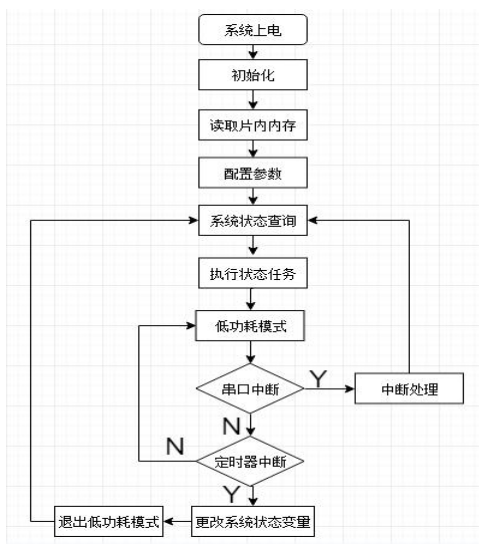
\includegraphics[width=0.6\textwidth]{fig/系统流程图.png}
	\caption{系统流程图}
	\label{fig:系统流程图}
\end{figure*}

\subsection{系统配置}
在电子电路设计中将串口一用串口转USB芯片转化成了用于系统调试的USB接口。该接口主要用作系统参数的配置,还可以通过拟定指令查询系统的运行状态、提取备份数据等。

系统时间设置和定时时间设置都是微处理器通过SPI总线访问高精度实时钟芯片DS3234来实现的。时间和日历数据由写入适当的寄存器字节来设置和初始化。时间和日历寄存器的内容是BCD码格式。DS3234可以运行在24或者12小时模式。微处理器访问DS3234内部SRAM数据,进行读写时钟数据,即可获取到系统时钟。定时时间设置是通过DS3234的闹钟中断来实现的,设置闹钟时间为系统时间加上定时时长,每次系统时间与闹钟时间一致时,触发闹钟中断(DS3234的INT/SQW低电平有效)。系统的工作可分为两种,一种是正常工作模式,一种是定时模式,在定时模式下,系统会监测定时时间,达到定时时间则开始数据采集,在采样的周期之间系统会自动进入低功耗模式,可以下达Wake指令进行唤醒,也可以下达Sleep指令让系统随时进入低功耗模式。每次系统参数配置会保存下来,如需对参数进行清除可以下达Empty指令。系统配置指令如表~\ref{tab:系统配置指令}所示。
\begin{table*}[ht]
\caption{系统配置指令}
  \label{tab:系统配置指令}
\centering
    \begin{tabular}{|c|c|}
        \toprule
 {\bf 指令}&{\bf 说明}  \\      
%\bf表示字体加粗
        \hline
[TM=YYMMDD hhmmss]& \tabincell{c}{配置系统时间,YY代表 年,MM代表月,\\DD代表日,hh代表时,mm代表分,ss代表秒。} \\
%需要分行的单元格的语句用\tabincell{c}{所填写第一行内容\\第二行内容···},可以根据需要换行,也不限定换多少行。
        \hline
[cmd\_mod\_x]& \tabincell{c}{改变系统工作状态,x为0系统配置为正\\常模式,x为1系统配置为定时模式} \\
        \hline
SetTM=YYMMDD hhmmss& \tabincell{c}{配置定时时间,YY代表年,MM代表月,\\DD代表日,hh代表时,mm代表分,ss代表秒。} \\
        \hline
Empty& \tabincell{c}{清空系统的参数和flash} \\
     \hline
Wake& \tabincell{c}{系统唤醒} \\
     \hline
Sleep& \tabincell{c}{系统进入低功耗} \\
        \bottomrule
    \end{tabular}
\end{table*}
\subsection{独立看门狗设计}
为防止系统因外界环境干扰或不可预见的逻辑条件造成程序跑飞陷入死循环~\cite{hjm},软件上使用了独立看门狗设计,当独立看门狗IWDG被激活后,IWDG的计数器开始向下递减计数,当IWDG的计数器的值递减到0时,系统便会复位,为保证系统正常工作,必须在IWDG的计数器的值递减到0之前,重新给IWDG的计数器赋值。独立看门狗启动之后,在程序中便不能关闭,必须在规定时间内喂狗,否则将会产生一个复位信号导致系统重启。

独立看门狗这种设计的时钟源频率为40kHz,它采用LSI内部低速时钟,这种配置使得系统主时钟出现错误时,该时钟依旧能保持正常运行。独立看门狗初始化函数中,配置IWDG\_PR寄存器的值为0x06,即预分频系数prer设置为6,配置IWDG\_RLR寄存器的值为0xfff,即重装在值 rlr为 4095。溢出时间计算公式如式\ref{eq:times}:
\begin{equation}
\begin{split}
T_{out}=[(4\times(2^{prer})) \times rlr] /40 ms
\end{split}
\label{eq:times}
\end{equation}  

公式中T指代看门狗溢出时间,prer指代独立看门狗时钟预分频系数,rlr为独立看门狗的重装载值,可计算溢出时间为26.208s。由于RC振荡器频率不是一个精准的40kHz,实际值和理论值会有一定的偏差,故在系统软件设计中,必须预留足够的时间进行喂狗操作。当系统进入低功耗模式时,为防止系统因未喂狗而导致重启,软件上设置内部RTC闹钟中断,配置中断间隔为10s,在闹钟中断处理函数中会更改系统状态变量从而进入系统自检状态,在系统自检中进行喂狗操作。

\section{能源管理与控制模块}
能源管理与控制模块块的主要功能是,最大限度地减少电流的损耗,微处理器长期控制整个能源管理系统,在外部设备不工作时,切断其能源供应,并微处理器自身进入低功耗模式,系统时钟切换成低速外部时钟。
\subsection{电源管理设计}
低功耗海洋传感器集成系统在程序设计上,根据设定的采样周期获取海洋生态环境数据。系统各个外部部件的实际工作时间是很有限的,在外部部件的待机时间内,通过电源管理设计尽可能的减少待机时间功耗,用以达到低功耗设计的目标。

电源管理设计可以控制海洋传感器设备处于断电状态并且微处理器进入低功耗状态,这是控制系统能源消耗最佳的措施。上节介绍了定时时间的设置,当系统到达定时时间意味着要开始采集任务了。通过定时中断将微处理器从低功耗状态下唤醒,唤醒之后,微处理器命令给海洋传感器上电,然后海洋传感器接受下达的采集命令,最后海洋传感器进行数据采集任务。传感器的电源供应选择了可控式的DC/DC模块,其中的ctrl引脚连接到了微处理器的IO口上。

默认设置下,微处理器控制DC/DC模块处于断电的状态。在定时中断函数中,给对应ctrl引脚的IO口置位,即可完成给海洋传感器的上电。微处理器在设定的时刻可以通过中断来从低功耗模式进入到活跃模式,在周期性的活跃模式之间,微处理器皆会在LMP3低功耗模式下运行。电源管理流程图如图~\ref{fig:电源管理流程图}所示。
\begin{figure*}[ht]
    \centering
	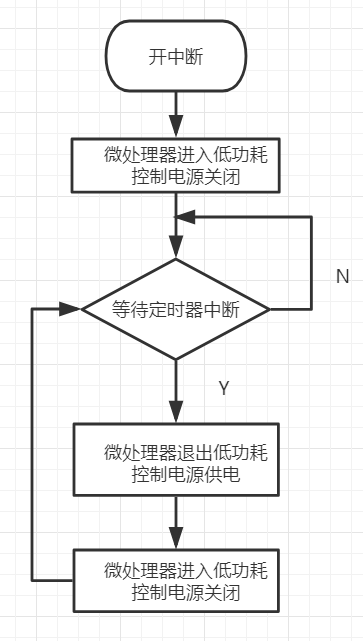
\includegraphics[width=0.5\textwidth]{fig/电源管理流程图.png}
	\caption{电源管理流程图}
	\label{fig:电源管理流程图}
\end{figure*}
\subsection{时钟切换设计}
微处理的功耗受到很多因素的影响,其中系统的运行频率是非常关键的影响要素。在关闭外部设备供电的情况下,MCU的功耗就主要取决于其系统时钟。

一般情况下,设计应选择尽可能小的运行频率。前文的硬件平台介绍提到,系统的时钟来源主要有两个:高速外部晶振电路(16MHz)和DS3234提供的低速32768Hz时钟。采用低速时钟作为系统运行频率,无疑会节省更多的能源损耗,但是考虑到系统处于活动模式下,微处理要参与完成众多的任务,比如与海洋传感器通信进行数据采集任务、与TF卡通信完成数据存储任务等,主系统MCLK为32768Hz时,系统的性能会大大的降低。所以根据系统实际应用的情况,要考虑到时钟的切换,即在系统正常工作的活跃状态下,要把微处理器的主系统时钟MCLK从LFXT1(外部低速晶振)切换到LFXT2(外部高速晶振),进入到低功耗模式下,微处理器只需维持基本的功能,等待中断将其唤醒,此时将系统时钟从高速切换回低速时钟。

% MSP430内部时钟图解如图~\ref{fig:MSP430时钟框架}所示。

% \begin{figure*}[ht]
%     \centering
% 	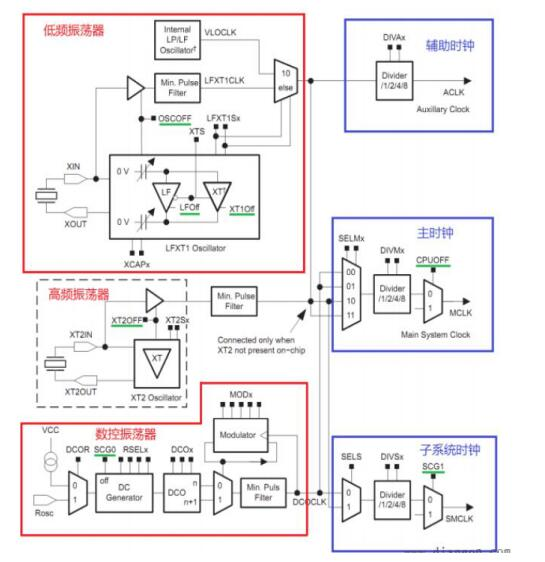
\includegraphics[width=0.7\textwidth]{fig/MSP430时钟框架.jpg}
% 	\caption{MSP430时钟框架}
% 	\label{fig:MSP430时钟框架}
% \end{figure*}

系统开启时,默认设置初始时钟为内部的DCO时钟。同时把XT1和XT2的功能都禁止了。但是DCO是内部集成的数字频率振荡器,其一内部的时钟频率不稳定,这会影响到系统的定时等功能,其二频率可能达不到性能要求。所以通常在使用时,都会切换到外部的晶体振荡器时钟。在本系统设计中,会涉及到这三种时钟的切换。比如,系统一上电后,初始时钟为默认的内部DCO时钟,然后进入低功耗模式下,时钟切换为外部低速时钟(32768Hz),需要执行采集任务时,系统处于活跃模式,时钟切换为高速外部时钟(16MHz)。

系统时钟主要通过修改BCSCTL1和BCSCTL2两个寄存器来配置。这两个寄存器的详细说明如图~\ref{fig:BCSCTL1寄存器}和图~\ref{fig:BCSCTL2寄存器}所示。
\begin{figure*}[ht]
    \centering
	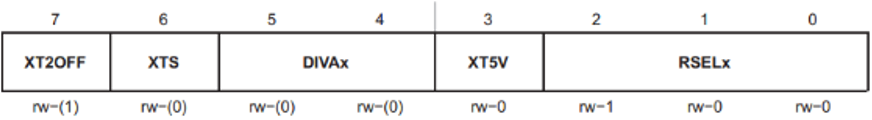
\includegraphics[width=1\textwidth]{fig/BCSCTL1寄存器.png}
	\caption{BCSCTL1寄存器}
	\label{fig:BCSCTL1寄存器}
\end{figure*}

XT2OFF:是否关闭高频振荡器。0开;1关。

XTS:选择低速晶体振荡器的工作方式。0为低;1为高。

\begin{figure*}[ht]
    \centering
	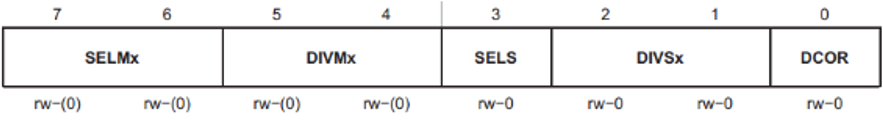
\includegraphics[width=1\textwidth]{fig/BCSCTL2寄存器.png}
	\caption{BCSCTL2寄存器}
	\label{fig:BCSCTL2寄存器}
\end{figure*}
SELMx:主系统时钟来源选择。

SELS:子系统时钟来源选择。

时钟来源要切换到外部时钟上去,一般需要进行几个步骤:

1)打开外部晶体振荡器,因为默认配置下XT1和XT2的功能是被禁止的。

2)清除晶体振荡器失效标志OFIFG标志。

3)等待50us,等待外部晶体振荡器工作。

4)监测晶振振荡器失效标志OFIFG标志,如果它没有失效,则外部晶体振荡器工作正常。

切换为XT2的程序代码实例如下:

\begin{lstlisting}[language=c++]
void ClokInit{
BCSCTL1&=~XT2OFF; //首先打开外部晶体振荡器。
 do{
    IFG1&=~OFIFG; //清除晶体振荡器失效标志OFFIFG标志
    for(int i=0xFF;i>0;i--); //等待50us,等待晶体振荡器正常工作
    }while((IFG1&OFIFG));//当OFFIFG等于0的时候结束,说明其正常工作。
BCSCTL2 |= SELM_2;
BCSCTL2 |= SELS;   //选择XT2时钟
}
\end{lstlisting}

\subsection{实时钟RTC设计}
低功耗海洋传感器集成系统的低速外部时钟直接是由高精度时钟芯片DS3234来提供的。一方面在电子电路设计中舍弃了外部晶振电路,简化电路设计和节省能源消耗;另外一方面为系统提供更加准确的时钟,这对于按点的电源管理和多参数数据的准同步都有重要的作用。通过设置DS3234的控制/状态寄存器来使能32KHz方波输出,控制/状态寄存器如图所示。

\begin{figure*}[ht]
    \centering
	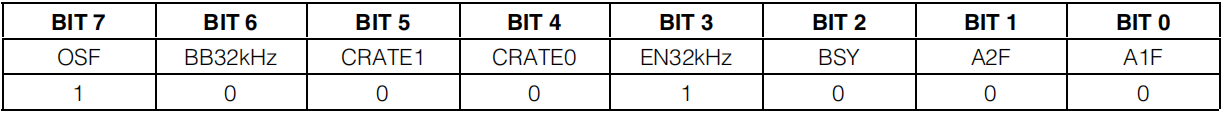
\includegraphics[width=1\textwidth]{fig/控制状态寄存器.png}
	\caption{控制状态寄存器.png}
	\label{fig:控制/状态寄存器}
\end{figure*}
位3是32KHz输出的使能,给位3置位时,输出一个32768Hz的方波输入。具体的操作是,微处理器通过SPI方式给控制状态寄存器(Ox0F)地址写入。
\section{数据采集与通信模块}
数据采集与通信模块的主要作用是,实现微处理器与海洋传感器之间的信息交互,比如微处理给传感器下达控制指令,传感器返回数据和状态信息等。
\subsection{串口中断软件设计}
数据采集与通信模块采集数据的方式是通过串口中断的方式实现的,同时预留的的调试接口都采取了中断的方式,当中断发生时,首先会对数据有效性进行判断,海洋观测数据以"*"开头,调试串口的数据以"["开头。每采集到一帧有效的海洋观测数据时,回复"[sendok]"表明接收成功并更改系统状态变量为Sava\_Data即数据存储状态,在主循环的系统状态检测中进入数据存储状态进行数据存储,存储成功后,相应的记录存储帧数的计数器将会加1,待发送数据帧数计数器也会加1,在系统自检状态检测到待发送数据帧数时将更改系统状态变量为Send\_Data即数据发送状态,在下一次系统状态检测中进入数据发送状态发送数据,数据发送成功时,对应的待发送数据帧数减1,已发送数据帧数加1,并将变量更新到系统状态表中并写入片内Flash的信息存储区,以便系统复位后对该信息重新获取。对于调试接口的数据,系统则对指令数据进行解析并执行对应的指令任务,任务完成后系统又进入到低功耗模式等到下一次中断的发生。串口中断程序流程图如图~\ref{fig:串口中断流程图}所示。

\begin{figure*}[ht]
    \centering
	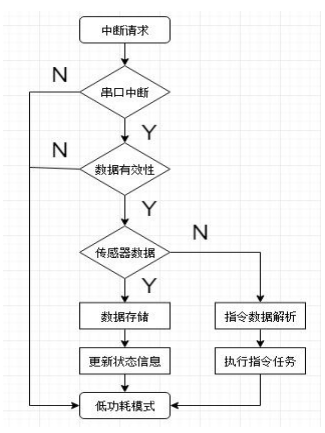
\includegraphics[width=0.7\textwidth]{fig/串口中断流程图.png}
	\caption{串口中断流程图}
	\label{fig:串口中断流程图}
\end{figure*}

\subsection{拓展串口软件设计}
针对微处理器现有的串口数量不足的问题,采用串口拓展芯片WK2124进行串口数量的拓展。微处理器是有多余的SPI总线接口的,所以在芯片选型时,选用可以实现SPI拓展4个串口功能的WK2124。SPI是串行外设接口,本质上是一个移位寄存器,将数据串行的输出到外围设备。通信原理主要以主从方式进行工作,可以实现一主多从工作模式。在本文中主要采用了主模块进行工作,即微处理器为主设备,串口拓展芯片为从设备,通常以四根线相连接进行通信,如表格~\ref{tab:SPI工作线}所示。

\begin{table}[htb]
  \centering\small
  \caption{SPI工作线}
  \label{tab:SPI工作线}
\begin{tabular}{|c|c|c|}
\hline
\multicolumn{2}{|c|}{\bf 名称}                  & {\bf 说明}                         \\ \hline
\multicolumn{2}{|l|}{MISO}                  & \multicolumn{1}{|c|}{主设备输入,从设备输出}                \\ \hline
\multicolumn{2}{|l|}{MOSI}                  & \multicolumn{1}{c|}{主设备输出,从设备输入}                \\ \hline
\multicolumn{2}{|l|}{SCLK}                  & \multicolumn{1}{c|}{时钟信号,由主设备产生}                         \\ \hline
\multicolumn{2}{|c|}{CS}                  & \multicolumn{1}{c|}{片选信号线,由主设备控制}                     \\ \hline
\end{tabular}
\end{table}

串口拓展芯片所通信的时钟主要由微处理器通过SCK引脚提供,再经由SPI的CS线选中需要进行数据传输任务的从设备。SPI的数据传输有着不同的总线协议模式,微处理器与WK2124必须配置相同的参数并使用相同的模式才能进行正常的通信,主要有两个参数决定SPI的传输方式:时钟极性和时钟相位,为芯片选择寄存器中的CPOL和CPHA位~\cite{2009zw},分别可取0或1,组成四种SPI工作模式,如表格~\ref{tab:SPI总线协议模式}所示。

%\newcommand{\tabincell}[2]{\begin{tabular}{@{}#1@{}}#2\end{tabular}}  
%表格自动换行
\begin{table*}[ht]
\caption{SPI总线协议模式}
  \label{tab:SPI总线协议模式}
\centering
    \begin{tabular}{|c|c|c|}
        \toprule
 {\bf SPI Mode}&{\bf CPOL} & {\bf CPHA}  \\      
%\bf表示字体加粗
        \hline
[0]& {0} & {0}\\
%需要分行的单元格的语句用\tabincell{c}{所填写第一行内容\\第二行内容···},可以根据需要换行,也不限定换多少行。
        \hline
[1]& {0} & {0}\\
\hline
[2]& {1} & {1}\\
\hline
[3]& {1} & {0}\\
        \bottomrule
    \end{tabular}
\end{table*}
SPI的四种工作模式区别主要是根据SCLK跳变沿进行数据采样~\cite{2006zxj},即在于是在SCLK的哪一位置进行数据传输任务,详细的工作原理和时序图分析不再赘述,具体可以参考数据手册和相关文档。

主设备MSP430F5438A微处理器通过SPI接口访问从设备WK2124,读取拓展串口采集的数据。WK2124工作在SPI同步串行通信的从机模式下,支持SPI模式0标准。为实现主机和WK2124的通信,在主机端需要设置CPOL=0(SPI时钟极性选择位),CPHA=0(SPI时钟相位选择位)。写FIFO操作,即给海洋传感器发送指令,先写入一个命令字节(Command Byte),随后写入相应的数据字节,FIFO地址自动增加。读FIFO操作,即接收海洋传感器采集数据,先写入一个命令字节(Command Byte),随后芯片SDOUT线上会返回相应的数据字节。FIFO地址自动增加。相关通信的流程图如图~\ref{fig:SPI通信流程图}所示。
\begin{figure*}[ht]
    \centering
	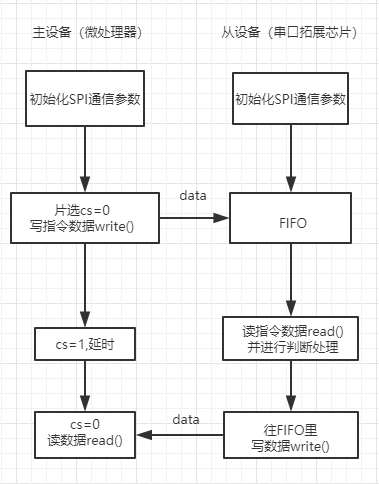
\includegraphics[width=0.6\textwidth]{fig/SPI通信流程图.png}
	\caption{SPI通信流程图}
	\label{fig:SPI通信流程图}
\end{figure*}

\subsection{传感器通信软件设计}
数据采集与通信模块最终的目标就是,通过微处理器本身的串口和拓展串口实现与海洋传感器的通信。各个海洋传感器与微处理器系统之间的通信方式主要是依靠RS232、RS285已经AML传感器本身的通信协议,中间主要是经过了相关电平信号的转换,所采集的数据才直接进入到微处理器当中。微处理器对于传感器下达的指令根据传感器类型的不同而不同,主要是对传感器的采样频率、时间校准、数据格式等进行相关配置,一般包括唤醒、开始采样和结束采样等命令,其中对于传感器的命令格式和详细配置在前面的章节均已介绍,下面主要是对命令转发到传感器的数据协议进行制定,如表格~\ref{tab:控制指令通信协议}所示。

%\newcommand{\tabincell}[2]{\begin{tabular}{@{}#1@{}}#2\end{tabular}}  
%表格自动换行
\begin{table*}[ht]
\caption{控制指令通信协议}
  \label{tab:控制指令通信协议}
\centering
    \begin{tabular}{|c|c|c|c|c|}
        \toprule
 {\bf 数据标号}&{\bf 字段名称} & {\bf 数据类型}& {\bf 数据长度} & {\bf 备注说明} \\      
%\bf表示字体加粗
        \hline
{\bf 1}& {包头} & {ASCII码}& {1 Byte} & \tabincell{c}{“*”-数据包的开始 }\\
\hline
%需要分行的单元格的语句用\tabincell{c}{所填写第一行内容\\第二行内容···},可以根据需要换行,也不限定换多少行。
{\bf 2}& {控制命令} & {ASCII码}& {不等} & \tabincell{c}{控制命令的内容和长度\\ 依据对应的传感器进行选取}\\
        \hline
{\bf 3}& {校验位} & {8 位无符号整数}& {1 Byte} & \tabincell{c}{对命令进行校验,默认为 0xff}\\
        \hline
{\bf 4}& {包尾} & {ASCII码}& {1 Byte} & \tabincell{c}{“*”-数据包的结束}\\
        \bottomrule
    \end{tabular}
\end{table*}

命令通过 RS232或485下发到传感器后,传感器会执行相关的指令,同时不同的传感器会将采集回来的数据传送到微控制器,其数据量比较大,且接收到的数据需要进行解析处理,所以需要单独分类,可以根据提前预定好的串口ID号来区分传感器,然后提取数据。对于返回数据量较大的传感器将预先设定足够大的缓冲区,可以通过自定义的队列结构暂存数据,然后按照时间节点进行传送。将按照表格~\ref{tab:数据包结构}的数据包结构进行数据采集。

%\newcommand{\tabincell}[2]{\begin{tabular}{@{}#1@{}}#2\end{tabular}}  
%表格自动换行
\begin{table*}[ht]
\caption{数据包结构}
  \label{tab:数据包结构}
\centering
    \begin{tabular}{|c|c|c|c|c|c|c|}
        \toprule
 {\bf 包头}&{\bf 相关信息} & {\bf 间隔}& {\bf 数据} & {\bf 间隔}& {\bf 校验}& {\bf 包尾} \\      
%\bf表示字体加粗
        \hline
{*}& {数据类型-\#-ID-\#-" 时间"} & {\#}& {数据体} & {\#}& {校验位}& {*}\\
        \bottomrule
    \end{tabular}
\end{table*}

除了包含主要的数据体外,还包括包头包尾、ID号、时间等必要的信息,其中ID主要是针对串口来事先定义好的标号,以此来区分不同的传感器。

\section{数据存储与回收模块}
数据储存与回收模块的主要作用是,系统的较长时间内采集的海洋水文数据都能够完整地进行存储,以便系统设备打捞上来后对数据进行回收备份。
\subsection{TF卡程序设计}
本次设计牺牲传输速率而选择了简便、速率稍低的SPI连接方式。上文介绍了SPI相关使用软件设计,本部分从TF卡程序设计进行阐述。

本次设计采用SPI总线与TF卡进行通信,需要首先进行的就是设置TF卡为SPI总线模式。具体的操作方法是:片选信号在复位命令来的时候处于有效的电平。由于TF内部供电电压上升需要一定的时间,这个时间大概是64个时钟左右,之后TF卡又要花费10时钟来进行卡同步,所以发送CMD0命令之前必须要等待74个时钟。TF卡初始化分为以下几个步骤:

1)初始化SPI接口及相关IO。通过SPI连接SD卡,所以先要初始化MCU的SPI接口,以及相关IO。

2)上电延时(>74个CLK)。 

3)卡复位(CMD0),进入IDLE状态。发送CMD0时,CS必须为低电平,使得SD卡进入SPI模式。

4)发送CMD8,检查是否支持SD卡2.0协议。

5)采用不同协议检查SD卡。

6)片选取消,结束初始化。

TF卡初始化流程图如图~\ref{fig:TF卡初始化流程}所示。
\begin{figure*}[ht]
    \centering
	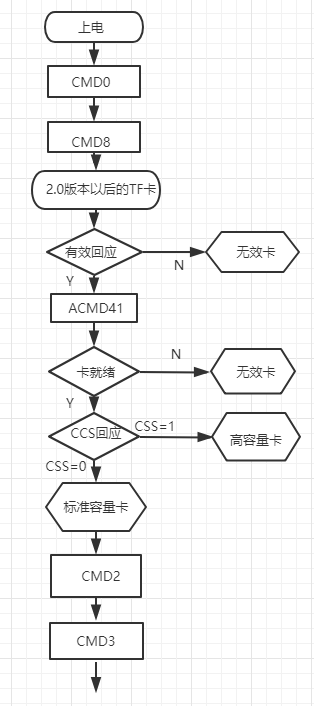
\includegraphics[width=0.5\textwidth]{fig/TF卡初始化流程.png}
	\caption{TF卡初始化流程}
	\label{fig:TF卡初始化流程}
\end{figure*}
\subsection{FATFS文件系统设计}
系统应用TF卡,需要文件系统管理进行协助。在众多的文件系统中,本文选择使用FATFS文件系统来管理TF卡。FATFS是一个完全用广泛认可的C语言编写的免费开源文件系统模块,硬件平台独立性使他优于其他文件模块,在移植到 8051、PIC、AVR、SH、Z80、H8、ARM等系列单片机时有较好的适用性,只需少量简单的修改。它支持多种存储格式和多个存储媒介;支持多个文件的读写操作。

FATFS的许多优点,以及它在软件开发上免费、开源的原则,使得FATFS应用非常广泛。FATFS模块的层次结构如图~\ref{fig:FATFS模块层次结构图}所示:

\begin{figure*}[ht]
    \centering
	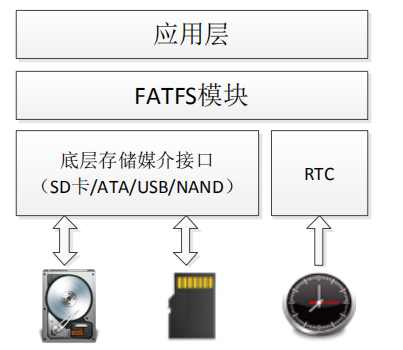
\includegraphics[width=0.5\textwidth]{fig/FATFS模块层次结构图.png}
	\caption{FATFS模块层次结构图}
	\label{fig:FATFS模块层次结构图}
\end{figure*}

如图~\ref{fig:FATFS模块层次结构图}所示,应用层直接给用户提供了丰富的接口函数,将它置于顶部,帮助用户简单使用而无需关注内部结构和协议等具体细节。中间层对文件的读写协议进行具体的要求,对于使用者不做修改要求,若需使用,将头文件进行引用便可。底层存储媒介接口需要进行代码编写移植的工作。

在进行FATFS移植之前,要做一些准备工作。在其官网获取FATFS软件包最新资源,解压获取到的资源包,得到doc和src两个文件夹。FATFS文件系统结构如图~\ref{fig:FATFS文件系统结构}所示。

\begin{figure*}[ht]
    \centering
	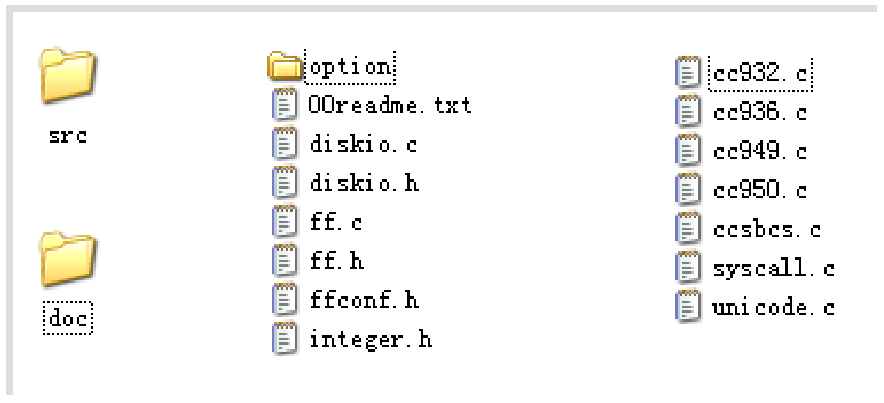
\includegraphics[width=0.7\textwidth]{fig/FATFS文件系统结构.png}
	\caption{FATFS文件系统结构}
	\label{fig:FATFS文件系统结构}
\end{figure*}

doc里面主要是对FATFS的介绍,而src里面是源码。硬件层包括diskio.c和diskio.h。文件系统的API层包括ff.c和ff.h。用户对ffcon.h和diskio.c进行修改配置,一般就能够完成移植的任务。ffconf.h里面包含了FATFS模块的所有配置信息和设置选项,可根据实际应用需求进行选择修改。diskio.c的主要功能是与底层硬件接口进行连接适配。这些文件的功能说明如表格~\ref{tab:FATFS文件系统包}所示。
%\newcommand{\tabincell}[2]{\begin{tabular}{@{}#1@{}}#2\end{tabular}}  
%表格自动换行
\begin{table*}[ht]
\caption{FATFS文件系统包}
  \label{tab:FATFS文件系统包}
\centering
    \begin{tabular}{|c|c|c|}
        \toprule
 {\bf 文件名}&{\bf 功能} & {\bf 说明} \\      
%\bf表示字体加粗
        \hline
 {ffconf.h}&{FATFS模块配置文件} & \tabincell{c}{需要根据需求\\来配置参数。} \\      
%\bf表示字体加粗
        \hline
 {ff.h}&{FATFS和应用模块公用的包含文件} & {不需要修改} \\      
%\bf表示字体加粗
        \hline 
 {ff.c}&{FATFS模块源码} & {不需要修改} \\      
%\bf表示字体加粗
        \hline
 {diskio.h}&{FATFS和disk I/O模块公用的包含文件} & {不需要修改} \\      
%\bf表示字体加粗
        \hline
{diskio.c}&{FATFS和disk I/O模块接口层文件} &\tabincell{c} {与平台相关的代码,\\需要用户根据存储介质来编写函数。} \\ 
%\bf表示字体加粗
        \hline
{interger.h}&{数据类型定义} & {与编译器有关。} \\ 
%\bf表示字体加粗
        \hline
{option文件夹}&{可选的外部功能(比如支持中文等)} & {根据应用环境} \\ 
        \bottomrule
    \end{tabular}
\end{table*}

移植FATFS文件系统的一般包括以下几个步骤:

1)数据类型:在integer.h里面去定义好数据的类型。这里需要了解你用的编译器的数据类型,并根据编译器定义好数据类型。

2)配置:通过ffconf.h配置FATFS的相关功能,以满足设计的需要。

3)函数编写:打开diskio.c,进行底层驱动编写,一般需要编写6个接口函数,如图~\ref{fig:diskio.c要实现的函数}所示。
\begin{figure*}[ht]
    \centering
	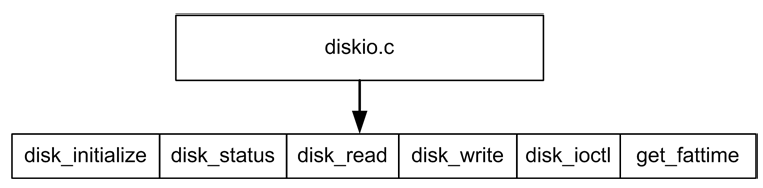
\includegraphics[width=0.7\textwidth]{fig/diskio.c要实现的函数.png}
	\caption{diskio.c要实现的函数}
	\label{fig:diskio.c要实现的函数}
\end{figure*}

通过软件设计部分将这六个函数一一实现,完成了对FATFS的移植之后,将可以在系统中正常的使用FATFS了。FATFS提供了很多API函数,在这里就不做过多的
赘述。建立好文件系统以后,首先建立一个数据文件夹(根据系统布放地点命名),然后根据日期来建立存储海洋水文数据的文件,每天生成一个TXT文件用来记录数据,如图~\ref{fig:水文数据文件}所示。
\begin{figure*}[ht]
    \centering
	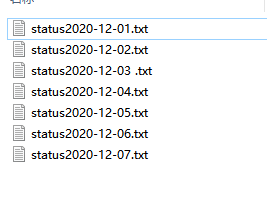
\includegraphics[width=0.5\textwidth]{fig/水文数据文件.png}
	\caption{水文数据文件}
	\label{fig:水文数据文件}
\end{figure*}

\section{本章小结}
在本章中主要针对低功耗海洋传感器集成系统的软件平台部分进行了详细的介绍,由于整个系统工作在海底环境,在软件设计上优先保障系统的低功耗性和 稳定性,首先介绍系统软件的设计原则,然后重点介绍和分析了四个功能模块的软件设计。
\chapter{实验测试与数据分析}
\label{cha:chapter6}
为了保证低功耗海洋传感器集成系统能够在低功耗指标下长期稳定的运行在海底环境中,在完成搭载平台的软硬件设计之后,需要对该平台进行集成实验测试,以保证平台的稳定性和可靠性。首先在实验室进行了模拟实验,对硬件平台的各部分功能模块进行了实验验证,对其中存在的错误和缺陷及时修改并补充,以达到所需的要求。之后将该平台在布放在海洋环境以完成实际的试验,最终实现海洋水文数据的采集和保存等功能。

\section{室内环境实验}
在将各个软硬件部分进行组装集成后,在实验室进行基本的功能和性能测试,以及低功耗、稳定性和可靠性测试。

主要是对传感器电源供电管理功能测试,包括上电和断电等功能、并对各传感器下达采样命令进行数据采集功能检测、传感器正常工作时的状态监测,包括电压和温度监控等、以及平台的整体运行性能等测试。通过多次实验证明,各传感器连接控制模块电压正常,能够为传感器做到正常上断电以及状态信息实时反馈,同时对传感器进行相关配置并下达采样命令后,将进行数据采集任务,通过串口将数据传送给微处理器,再对数据进行解析处理,最后通过TF卡将数据保存或者通过USB接口将数据回收。系统不需要进行采样时,微控制器进入低功耗模式,此时整个系统处于休眠状态。对于仅依靠于电池组供电的系统来说,休眠状态大大节省了电池电量,延长了系统在海洋环境下的生存时间。

在实验室经过30天稳定运行后,对于传感器电源管理、低功耗模式以及数据采集等功能均能正常平稳进行,平台的整体功能及性能基本可以达到投放条件。同时经过反复实验检测,对其中出现的问题做到及时反馈分析并解决,并且对平台的软硬件部分功能进行优化和改进设计,以最终满足整体布放和业务化运行条件。

水密控制舱和系统平台框架搭建完成后的室内环境测试实验具体分为三个部分:耗电测试、命令测试和数据测试。
\subsection{耗电测试}
为了测试系统具体的低功耗性能指标,通过预留的USB接口连接到个人电脑,使用串口调试助手,给微处理器发送系统交互的命令进行电源控制,在供电电压在12V的情况下,采用高精度数字直流电源,记录各部件耗电情况。通过微处理器控制给所有的外部部件断电,测得的即是MCU单元电流,然后分别控制MCU进入活跃状态和低功耗状态,得到不同工作模式下MCU单元的电流,依次控制给各个部件上电,测量其电流大小,各部件耗电电流如表格~\ref{tab:各部件耗电情况}所示。

%\newcommand{\tabincell}[2]{\begin{tabular}{@{}#1@{}}#2\end{tabular}}  
%表格自动换行
\begin{table*}[ht]
\caption{各部件耗电情况}
  \label{tab:各部件耗电情况}
\centering
    \begin{tabular}{|c|c|c|c|}
        \toprule
 {\bf 部件名称}&{\bf 部件功耗/mA} & {\bf 每小时工作时长/s} & {\bf 每日平均功耗/Ah}\\    
%\bf表示字体加粗
        \hline
 {活跃状态MCU单元}&{5mA} & {3600}&{0.12}\\      
%\bf表示字体加粗
        \hline
 {低功耗状态MCU单元}&{可忽略} & {3600}&{可忽略}\\      
%\bf表示字体加粗
        \hline
 {MAX232CSE芯片}&{1mA} & {3600}&{0.024}\\      
%\bf表示字体加粗
        \hline
 {串口拓展芯片WK2124}&{3mA} & {3600}&{0.072}\\      
%\bf表示字体加粗
        \hline
 {时钟芯片DS3234}&{2mA} & {3600}&{0.036}\\      
%\bf表示字体加粗
        \hline
{CH340E芯片}&{1mA} & {3600}&{0.024}\\      
%\bf表示字体加粗
        \hline
{TF卡模块}&{30mA} & {60}&{0.012}\\      
%\bf表示字体加粗
        \hline
{AML系列传感器(温盐)}&{72mA} & {60}&{0.029}\\      
%\bf表示字体加粗
        \hline
{溶解氧传感器}&{48mA} & {60}&{0.019}\\      
%\bf表示字体加粗
        \hline
    \end{tabular}
\end{table*}
表格~\ref{tab:各部件耗电情况}列举的各部件耗电占据了系统能源消耗绝大部分,其余的一些外部部件,由于耗电非常低,几乎可以对其进行忽略。按照目前完成的实验室测试数据,系统集成4个AML系列海洋传感器和1个溶解氧传感器,每个小时传感器采集一分钟数据,然后进行数据存储的情况下,一天内的总功耗大约是0.442/Ah,本设计使用七节锂电池串联组作为接入电源,锂电池的容量为95Ah,运行天数是215天。实际的应用中,海洋传感器集成数量和采集周期的不同,都会导致系统有效工作时长会发生变化。
\subsection{命令测试}
进行命令测试,目的是确保设备的功能性、稳定性。一般向海洋传感器长时间反复发送一些常用的命令,可以检查出电气连接和功能是否有问题。

1)查看目前串口通信的传感器探头类型,可以发送VERSION命令,串口将会接收到传感器反馈回来的版本信息如图~\ref{fig:VERSION命令}所示。

\begin{figure*}[ht]
    \centering
	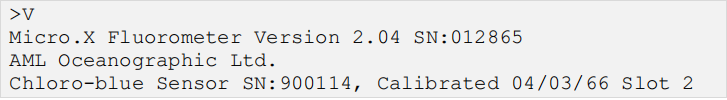
\includegraphics[width=1\textwidth]{fig/VERSION命令.png}
	\caption{VERSION命令}
	\label{fig:VERSION命令}
\end{figure*}

2)一些重要的设置命令测试,比如设置串口的波特率和传感器的采样频率。

串口通信必须约定双方使用相同的波特率。设置波特率的命令是SET DETECT ab,b可以是1到9的数字。 

数字所对应的波特率如下所示:

\begin{lstlisting}
1 = 600
2 = 1200
3 = 2400
4 = 4800
5 = 9600
6 = 19200
7 = 38400
8 = 57600
9 = 115200
\end{lstlisting}

每次在使用串口通信的波特率配置时,根据系统所需要的波特率,去找到数字所对应的波特率即可。如图~\ref{fig:波特率设置命令}所示的命令表示将串口波特率设置为38400(b=7)。在本次设计中一般使用9600的波特率,直接将b代表的数字改成6就可完成波特率设置。

\begin{figure*}[ht]
    \centering
	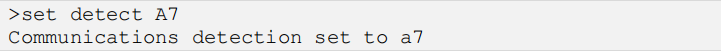
\includegraphics[width=1\textwidth]{fig/波特率设置命令.png}
	\caption{波特率设置命令}
	\label{fig:波特率设置命令}
\end{figure*}

采样率是传感器配置的关键参数之一,决定了传感器的采样速率,AML系列的海洋传感器具有采样速率高的特点,最高速率可达每秒25个样本。SET SAMPLE RATE n t(简写为SET S)是设置采样率的命令,其中n t有不同的表示方法,这样对于用户使用来说更加灵活,既可以设置为采样率,也可以用采样周期来表示,如下所示:

\begin{lstlisting}
n /S:将采样率设置为每秒n个样本。
n /M:将采样率设置为每分钟n个样本。
n /H:将采样率设置为每个小时n个样本。
n S:样本的采样周期设置为n秒。
n M:样本的采样周期设置为n分钟。
n H:样本的采样周期设置为n小时。
\end{lstlisting}

如图~\ref{fig:采样率设置命令}所示的命令分别表示样本采样周期为一秒和采样率为每秒一个样本。

\begin{figure*}[ht]
    \centering
	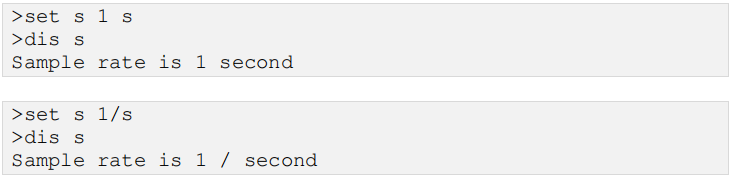
\includegraphics[width=1\textwidth]{fig/采样率设置命令.png}
	\caption{采样率设置命令}
	\label{fig:采样率设置命令}
\end{figure*}

3)接下来测试采样命令SCAN(简写为S)和MONITOR(简写为M).它们的区别是:SCAN是输出一次数据扫描,MONITOR是流数据按设置的采样率输出。

\begin{figure*}[ht]
    \centering
	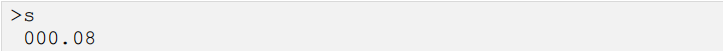
\includegraphics[width=1\textwidth]{fig/SCAN命令.png}
	\caption{SCAN命令}
	\label{fig:SCAN命令}
\end{figure*}

如图~\ref{fig:SCAN命令}所示,SCAN命令进行了一次采样。

\begin{figure*}[ht]
    \centering
	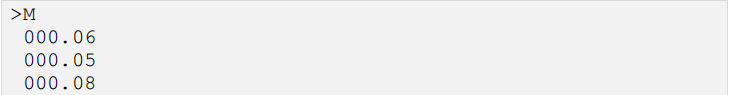
\includegraphics[width=1\textwidth]{fig/MONITOR命令.png}
	\caption{MONITOR命令}
	\label{fig:MONITOR命令}
\end{figure*}

如图~\ref{fig:MONITOR命令}所示,MONITOR命令进行按采样率进行连续采样。

命令测试主要是为了测试系统功能性和稳定性,在功能性上使用串口调试助手等工具对低功耗海洋传感器系统反复下达控制指令,比如微处理工作模式选择和切换以及海洋海洋传感器进行上电、断电、命令下达等功能性测试,以上操作都能准确执行。在进行稳定性的测试过程中,整个系统的软硬件平台均能连续稳定工作30天以上,符合稳定性测试要求。

\subsection{数据测试}
数据测试的主要作用是保证系统通过海洋传感器采集而来的数据具有现实意义和研究价值。室内环境,要测试微处理器控制板在连接不同的传感器探头情况下,采集水文数据,其数据的有效性。利用控制变量的实验方法对采样数据进行对比分析。

1.对Smart Turbidity(浊度)传感器进行测试。

测试方法:用杯子取半杯自来水,水量恰好满过传感器,进行数据采样,如图~\ref{fig:浊度传感器测量自来水}所示。
\begin{figure*}[ht]
    \centering
	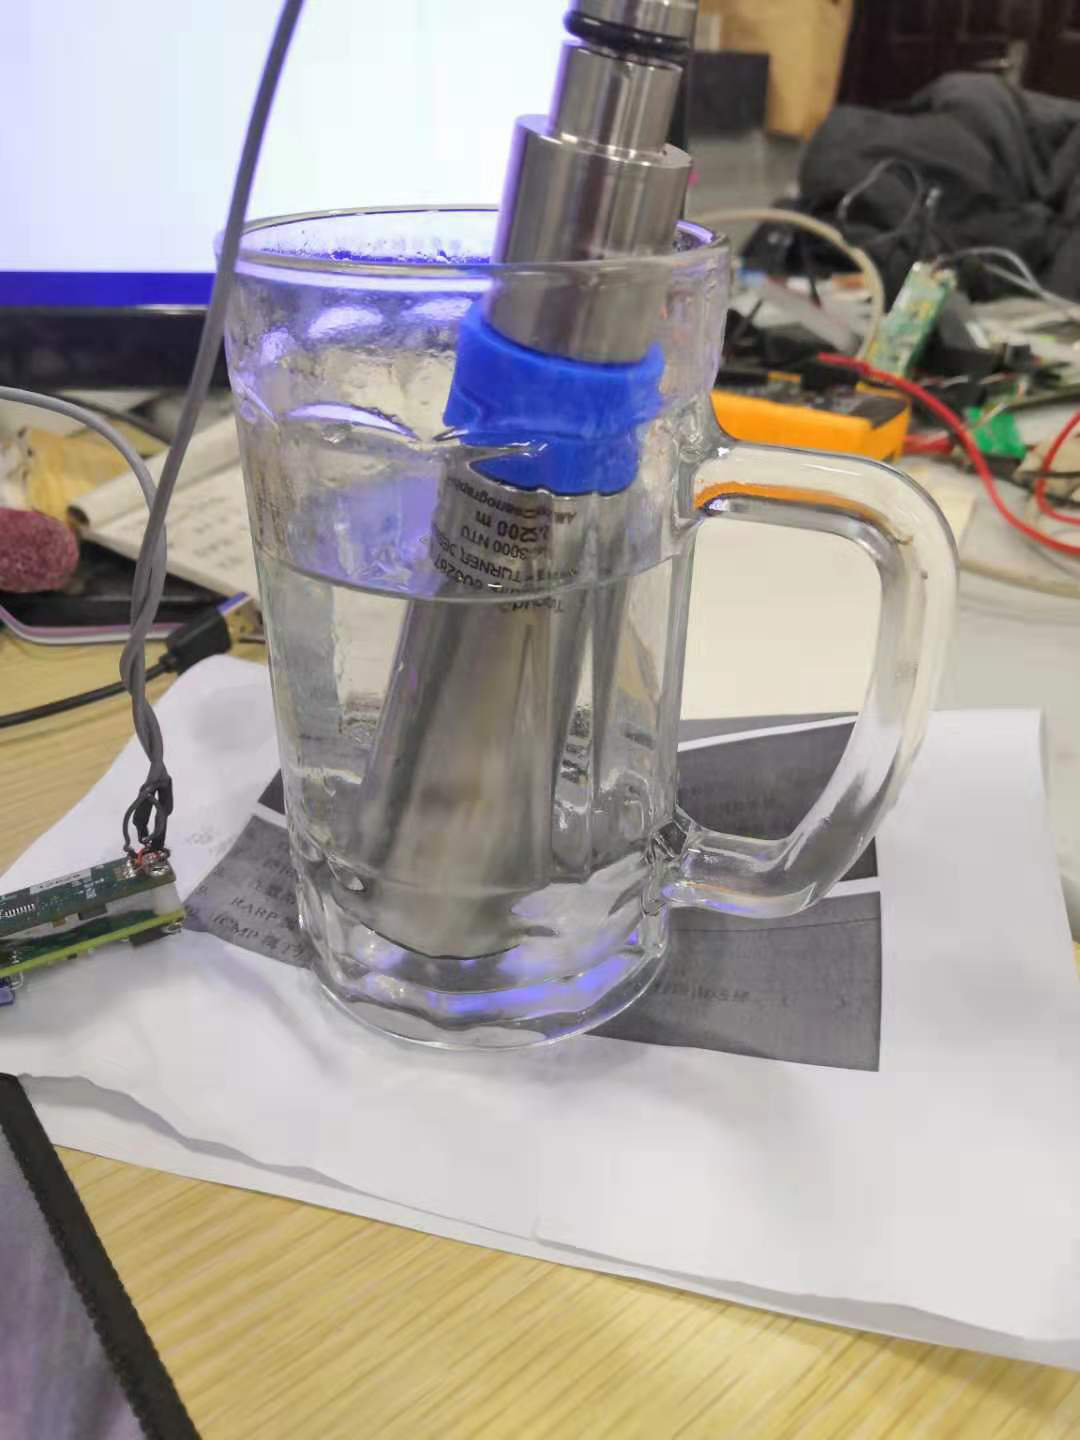
\includegraphics[width=0.4\textwidth]{fig/浊度传感器测量自来水.png}
	\caption{浊度传感器测量自来水}
	\label{fig:浊度传感器测量自来水}
\end{figure*}

之后往水杯中加入几毫升牛奶,摇晃均匀后采样,如图~\ref{fig:浊度传感器测量混有牛奶的自来水}所示。

\begin{figure*}[ht]
    \centering
	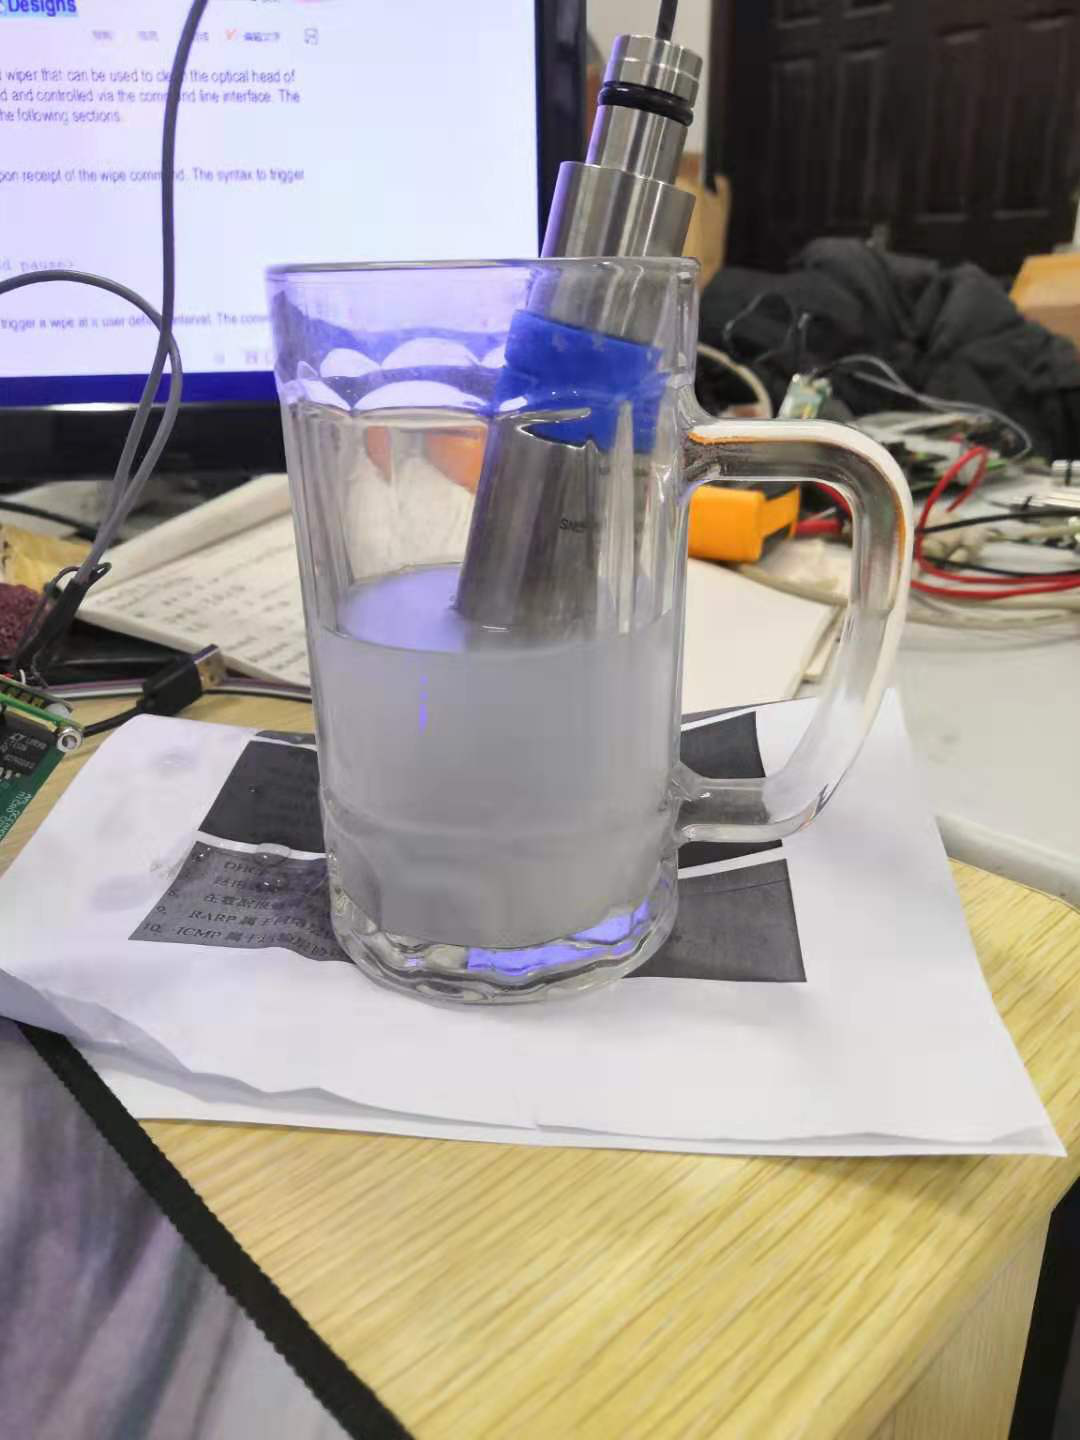
\includegraphics[width=0.4\textwidth]{fig/浊度传感器测量混有牛奶的自来水.png}
	\caption{浊度传感器测量混有牛奶的自来水}
	\label{fig:浊度传感器测量混有牛奶的自来水}
\end{figure*}

智能浊度传感器在监测时传输两个数据通道,测量通道和状态通道。测量通道包含传感器收集的测量数据。由于智能浊度传感器配有驱动雨刷,可用于清洁探头的气泡、微生物或碎片。状态通道指示每次测量是否可靠。测量可能已被雨刷的活动损坏。状态为0表示可靠数据,而状态为1表示测量可能受到雨刷活动的强烈影响。

表~\ref{tab:浊度}列举了智能浊度传感器在自来水和牛奶溶液下分别三次采样数据,在不受雨刷影响下对两种溶液所测量得到的数据差异很大,同一溶液之间的三次采样误差很小。
\begin{table}[ht]
\caption{浊度传感器对两种不同浊度溶液的三次采样}
\label{tab:浊度}
\centering
    \begin{tabular}{|c|c|c|c|}
        \hline
        \diagbox{溶液}{采样编号} & 第一次 & 第二次&第三次 \\   
        %斜线命令语句
        \hline
        自来水 &0005.05 0&0005.04 0 &0005.14 0\\
         \hline
        混有牛奶的自来水 & 0339.35 0 &0339.57 0&0339.36 0\\
         \hline
    \end{tabular}
\end{table}

2.对CT(盐度和温度)传感器进行测试。

测试方法:用杯子取半杯自来水,水量恰好满过传感器,进行数据采样,然后将杯子内的自来水倒出少许,换成热水采样,最后将杯子内的自来水换成标准海水采样。由于CT传感器具有两种参数,设置了两组对照试验来对比。

CT传感器在监测时传输两个数据通道。一个通道输出电导率数据(反应出盐度参数),另一个通道输出温度数据。

\begin{table}[ht]
\caption{CT传感器对三种不同溶液的三次采样}
\label{tab:CT•Xchange}
\centering
    \begin{tabular}{|c|c|c|c|}
        \hline
        \diagbox{溶液}{采样编号} & 第一次 & 第二次&第三次 \\   
        %斜线命令语句
        \hline
        自来水 &00.967 19.860&00.965 19.860&00.967 19.858\\
         \hline
        温水 & 00.909 23.897&00.911 23.894&00.912 23.892\\
         \hline
        标准海水 & 42.356 19.951&42.361 19.955&42.362 19.959\\
         \hline
    \end{tabular}
\end{table}

表格~\ref{tab:CT•Xchange}列举了CT传感器对自来水、温水、海洋三种不同溶液的三次采样数据,可以看到自来水和温水之间有温度数据上的差异,在采样的同时,使用温度计对两种溶液温度进行了测定,在温度数据上与CT传感器采集温度数据差异很小,而自来水和标准海水之间在盐度数据上的差异较大,这符合常规认知。


3.对Smart pH传感器进行测试。
测试方法:用杯子取半杯自来水,水量将将满过传感器。将杯子内的自来水换成标准海水。对比不同PH值的水采样数据的差异。

\begin{table}[ht]
\caption{Smart pH传感器对两种不同溶液的三次采样}
\label{tab:PH}
\centering
    \begin{tabular}{|c|c|c|c|}
        \hline
        \diagbox{溶液}{采样编号} & 第一次 & 第二次&第三次 \\   
        %斜线命令语句
        \hline
        自来水 &06.40&06.3 & 06.2\\
         \hline
        标准海水 & 06.7 &06.7&06.7\\
         \hline
    \end{tabular}
\end{table}

从表格~\ref{tab:PH}中看到,采样的自来水和标准海洋的PH数据差异并不大,经过查阅互联网资料发现这两种溶液PH值是有可能出现相近的情况。

4.对Smart Chlorophy (叶绿素)传感器进行测试。
测试方法:用杯子取半杯自来水,水量将将满过传感器。将杯子中的自来水换成从河道取来的河水。对比不同叶绿素含量的水采样数据的差异。

\begin{table}[ht]
\caption{Smart Chlorophy传感器对两种不同溶液的三次采样}
\label{tab:chl}
\centering
    \begin{tabular}{|c|c|c|c|}
        \hline
        \diagbox{溶液}{采样编号} & 第一次 & 第二次&第三次 \\   
        %斜线命令语句
        \hline
        自来水 &000.26&000.24 & 000.26\\
         \hline
        河道水 & 020.50 &021.55&021.65\\
         \hline
    \end{tabular}
\end{table}

从表格~\ref{tab:chl}中看到,河道水中叶绿素的含量比自来水丰富很多,河道水的叶绿素反应了藻类的浓度较高,自来水经过消毒,其藻类浓度自然很低。

5.对UV灯进行测试。
测试方法:设置亮灭时间分别为一分钟和两分钟,然后用手机秒表计数。
\begin{table}[ht]
\caption{UV灯定时闪烁测试}
\label{tab:UV}
\centering
    \begin{tabular}{|c|c|c|c|}
        \hline
        \diagbox{时长}{采样编号} & 第一次 & 第二次&第三次 \\   
        %斜线命令语句
        \hline
        60S &\tabincell{c}{灭-59.45s  \\ 亮-60.15s}&\tabincell{c}{灭-59.65s \\ 亮-60.25s}&\tabincell{c} {灭-59.55s \\  亮-60.15s}\\
         \hline
        120S&\tabincell{c}{灭-119.75s \\   亮-119.15s}&\tabincell{c}{灭-120.65s \\  亮-120.25s}& \tabincell{c}{灭-119.55s \\  亮-120.15s}\\
         \hline
    \end{tabular}
\end{table}

表格~\ref{tab:UV}通过秒表计时时间与设置的闪烁时间进行对比,可知UV灯的功能是基本正常的。
\section{室外环境实验}
室内环境实验测试完成后,为了确保系统在室外海域环境下能达到长期稳定运行的要求,接下来需进行外部环境测试。为了模拟海洋的实际环境提高实验的仿真性,对低功耗海洋传感器集成系统进行了为期30天的浅海选址、布放、回收的试验。经过为期30天的浅海测试分析,低功耗海洋传感器集成系统的各部分软硬件都能稳定的工作,传感器进行能源管理、数据采集和命令下达控制,修改各传感器采样配置方案等操作均正常工作。综上所述,系统已达到长期稳定运行的要求。外部环境布放如图~\ref{fig:外部环境测试效果图}所示。

\begin{figure*}[ht]
    \centering
	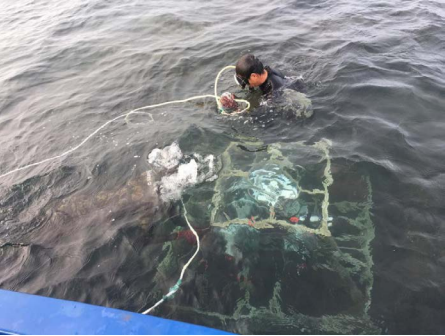
\includegraphics[width=0.7\textwidth]{fig/外部环境测试效果图.png}
	\caption{外部环境布放图}
	\label{fig:外部环境测试效果图}
\end{figure*}

\section{实验数据分析}
多参数水质仪采样的数据包括水位、海水温度、盐度、溶解氧、叶绿素、浊度、PH。经过30天的布放使用和观察,现对第1周采集的数据进行汇总和分析,大致总结了如下数据的变化趋势。

浅海测试海域的潮汐变化以潮周期变化为主,最高水位18m左右,最低水位15m左右,高低水位差3m左右,平均水位在16.5m,变化范围在0.5-1.3m之间。经过第1 周的潮汐高低的水位变化的观察,存在高水位较高、最低水位较高的现象,故将浅海海域判定为不正规全日潮类型。在水温监测方面,7天的时间整体气温呈明显的下降趋势,存在3天时间有小幅升温。观测过程中平均水温29.1℃,平均日温差 12℃。在盐度监测方面,由于浅海海域温度相对稳定,近海岸海水盐度变化较小,7天观测期未出现明显波动。观测时间段内平均盐度为32.06,标准差在0.0016,盐度较为均匀。在溶解氧监测方面,平均浓度为6.46mg/L,日变化幅度在0.3-0.5mg/L之间,标准差为0.0061mg/L。在叶绿素监测方面,在观测期间的第4天出现峰值,其余时间变化幅度相对稳定,叶绿素浓度平均值为0.232μg/L,浓度标准差约为0.0016μg/L。在浊度监测方面,观测值在后3天增长趋势较大,7天内的浊度平均值为0.873,标准差位0.0652,相对于温度、盐度、叶绿素三个数据浊度变化幅度较大。在PH值监测方面,在第4日至第7日上升幅度较大,7天内PH平均值为8.213,标准差为0.0006。以上信息汇总如图~\ref{fig:测试数据}所示。

\begin{figure*}[ht]
    \centering
	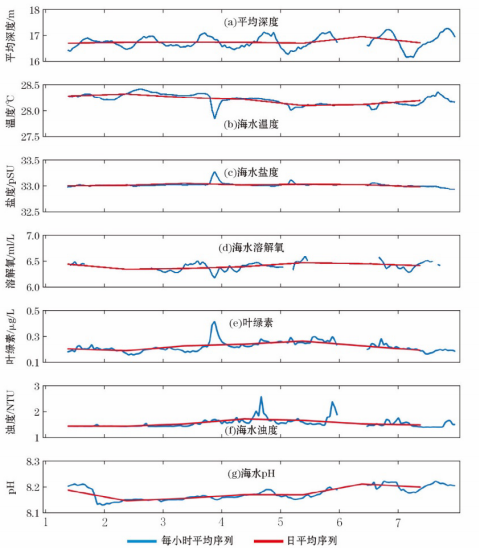
\includegraphics[width=1\textwidth]{fig/浅海测试第1周海洋水文数据曲线图.png}
	\caption{浅海测试第1周海洋水文数据曲线图}
	\label{fig:测试数据}
\end{figure*}

\section{本章小结}
在完成系统整体架构设计和系统的软硬件设计后,先后进行了水密控制舱和平台整体框架的组装。为了保证系统实际布放后可以长期稳定的运行,依次进行系统通信速率测试、功能稳定测试的室内环境实验和为期30天浅海的外部环境实验,经测试和分析海洋水文数据、海洋动力数据,初步认定低功耗海洋传感器集成系统符合功能性和稳定性的要求,可在海洋环境布放设备并陆续开展实际数据采集工作。
\chapter{总结与展望}
\label{cha:chapter7}

\section{总结}
本文主要提供了一个海洋生态环境监测的实现方案,采用集成式管理方式,设计了低功耗海洋传感器集成系统的主体结构,重点讲述了系统平台的低功耗设计、硬件设计和软件设计,阐明了电源的有效控制、传感器连接控制以及数据采集中心和部分电路原理图,整体具有功耗低、结构清晰、开发周期短等优点。系统选取了合适的超低功耗微处理器MSP430系列来作为控制核心,并完成相关硬件平台搭建,通过软件平台控制来完成传感器的数据采集以及电源管理等任务,最终海洋水文数据的有效采集和本地保存等功能。系统整体运行稳定,通过海洋环境的实地布放,可以对海洋生态环境的变化实现长期稳定的监测,能够达到预期的效果。

本文主要完成了以下工作:

(1)首先介绍了完整的低功耗海洋传感器集成系统总体设计方案,并重点剖析了海洋传感器的整体架构以及微处理系统的设计框图。采用MSP430微处理器进行电源控制,通过定点启动电源来触发采集任务,当平台数据采集任务处于上一个工作周期与下一个工作周期的中间休眠期时,将关闭电源,使微微处理器与传感器等外部设备可以在间歇时刻休息,以此来进一步降低平台的功耗,保证了能源消耗的最小化。一般的传感器集成系统只是简单的设计多个接口,不同的传感器类型之间很难实现替换,本系统不同传感器之间替换,只需更换探头即可实现。设计了两种通信接口协议,既能保证一般使用RS232协议的传感器可进行连接,又能连接使用专门AML接口协议的传感器。在已有的硬件资源基础之上,通过串口拓展芯片可随时增加连接传感器个数,使得系统具备可拓展性。在可靠性方面数据本地保存采用了冗余设计,分别对两片存储单元进行读写,保证了平台数据的稳定性,最终提升系统的整体工作性能。

(2)MSP430系列超低功耗微处理器是低功耗海洋传感器集成系统的硬件核心,围绕着它讨论了多种的低功耗设计方案。首先在嵌入式微处理器选型上,综合比较了C8051系列、STM32系列和MSP430系列,在实现性能的条件下,MSP430是能源节省和高效控制的最优选择。其次从电源管理方法上,具体分析了系统电源管理,比如电源在不同模式下的开启和关闭,时钟工作频率在不同模式的切换。

(3)由于整个传感器集成系统只有一个任务处理中心,且传感器的数据采集过程以及状态管理的数据反馈等所有的工作任务重担将全部交给微处理器进行处理。在软件平台设计上,分模块进行程序设计,通过系统管理与配置模块和数据采集与通信模块,分别实现与管理人员、海洋传感器之间的信息交互。能源管理与控制模块的软件设计实现了电源的有效控制,数据存储和回收模块对海洋生态环境数据进行有效的保存和处理。

本文主要以集成式管理方式实现对海洋生态环境的数据采集任务,通过布放于海洋环境进行实验验证,能够完成相关工作任务,为海洋环境监测和保护领域提供了一套新的解决方案。
% 文献引用~\cite{he2016deep}

\section{展望}
%新的一天快快把论文写完! 回来亲亲我的宝贝!

本文中的低功耗传感器集成系统能够满足基本要求,可以实现海洋生态环境数据的采集、储存和回收等工作,并且能够在海域中长期稳定的运行,但由于时间关系和作者掌握知识的局限性,后期可以从以下方面对平台加以改进,使平台功能更加完善可靠。

\subsection{电源控制升级}
由于海边环境的复杂性以及天气等原因,为了进一步保护传感器集成系统的安全,可中加入电压采集模块,以此来监测系统最开始处的电源供应或转换部分的电压变化。在单片机的程序中设定电压阈值,当电压出现较大的波动时且在无人值守的情况下,将启动电源切断程序,直接从电源供应或转换处切断能源供给,进一步加强对系统的保护,避免因电压波动所带来的破坏。

\subsection{便捷化和小型化}
海洋观测系统往便捷化、小型化发展是必然趋势。可通过电路板的PCB布局、更小型的封装、多层板结合的方式缩小电路板的体积,同时在硬件软件设计上进一步降低系统的功耗,从而减少携带的电池量,大大减少舱体的体积和重量。

%%% 其它部分
% \backmatter

%% 本科生要这几个索引,研究生不要。选择性留下。
% 插图索引
% \listoffigures
% 表格索引
% \listoftables
% 公式索引
% \listofequations


%% 参考文献
% 注意:至少需要引用一篇参考文献,否则下面两行可能引起编译错误。
% 如果不需要参考文献,请将下面两行删除或注释掉。
\bibliographystyle{thuthesis}
% \clearpage %目录中显示的页码正确
% \phantomsection %目录中的链接能正确跳转
% \addcontentsline{toc}{chapter}{参考文献} %目录中以章的名义添加条目
\bibliography{ref/refs}


%% 附录
% \begin{appendix}
% \chapter{外文资料原文}
\label{cha:engorg}

\title{The title of the English paper}

\textbf{Abstract:} As one of the most widely used techniques in operations
research, \emph{ mathematical programming} is defined as a means of maximizing a
quantity known as \emph{bjective function}, subject to a set of constraints
represented by equations and inequalities. Some known subtopics of mathematical
programming are linear programming, nonlinear programming, multiobjective
programming, goal programming, dynamic programming, and multilevel
programming$^{[1]}$.

It is impossible to cover in a single chapter every concept of mathematical
programming. This chapter introduces only the basic concepts and techniques of
mathematical programming such that readers gain an understanding of them
throughout the book$^{[2,3]}$.


\section{Single-Objective Programming}
The general form of single-objective programming (SOP) is written
as follows,
\begin{equation}\tag*{(123)} % 如果附录中的公式不想让它出现在公式索引中,那就请
                             % 用 \tag*{xxxx}
\left\{\begin{array}{l}
\max \,\,f(x)\\[0.1 cm]
\mbox{subject to:} \\ [0.1 cm]
\qquad g_j(x)\le 0,\quad j=1,2,\cdots,p
\end{array}\right.
\end{equation}
which maximizes a real-valued function $f$ of
$x=(x_1,x_2,\cdots,x_n)$ subject to a set of constraints.

\newtheorem{mpdef}{Definition}[chapter]
\begin{mpdef}
In SOP, we call $x$ a decision vector, and
$x_1,x_2,\cdots,x_n$ decision variables. The function
$f$ is called the objective function. The set
\begin{equation}\tag*{(456)} % 这里同理,其它不再一一指定。
S=\left\{x\in\Re^n\bigm|g_j(x)\le 0,\,j=1,2,\cdots,p\right\}
\end{equation}
is called the feasible set. An element $x$ in $S$ is called a
feasible solution.
\end{mpdef}

\newtheorem{mpdefop}[mpdef]{Definition}
\begin{mpdefop}
A feasible solution $x^*$ is called the optimal
solution of SOP if and only if
\begin{equation}
f(x^*)\ge f(x)
\end{equation}
for any feasible solution $x$.
\end{mpdefop}

One of the outstanding contributions to mathematical programming was known as
the Kuhn-Tucker conditions\ref{eq:ktc}. In order to introduce them, let us give
some definitions. An inequality constraint $g_j(x)\le 0$ is said to be active at
a point $x^*$ if $g_j(x^*)=0$. A point $x^*$ satisfying $g_j(x^*)\le 0$ is said
to be regular if the gradient vectors $\nabla g_j(x)$ of all active constraints
are linearly independent.

Let $x^*$ be a regular point of the constraints of SOP and assume that all the
functions $f(x)$ and $g_j(x),j=1,2,\cdots,p$ are differentiable. If $x^*$ is a
local optimal solution, then there exist Lagrange multipliers
$\lambda_j,j=1,2,\cdots,p$ such that the following Kuhn-Tucker conditions hold,
\begin{equation}
\label{eq:ktc}
\left\{\begin{array}{l}
    \nabla f(x^*)-\sum\limits_{j=1}^p\lambda_j\nabla g_j(x^*)=0\\[0.3cm]
    \lambda_jg_j(x^*)=0,\quad j=1,2,\cdots,p\\[0.2cm]
    \lambda_j\ge 0,\quad j=1,2,\cdots,p.
\end{array}\right.
\end{equation}
If all the functions $f(x)$ and $g_j(x),j=1,2,\cdots,p$ are convex and
differentiable, and the point $x^*$ satisfies the Kuhn-Tucker conditions
(\ref{eq:ktc}), then it has been proved that the point $x^*$ is a global optimal
solution of SOP.

\subsection{Linear Programming}
\label{sec:lp}

If the functions $f(x),g_j(x),j=1,2,\cdots,p$ are all linear, then SOP is called
a {\em linear programming}.

The feasible set of linear is always convex. A point $x$ is called an extreme
point of convex set $S$ if $x\in S$ and $x$ cannot be expressed as a convex
combination of two points in $S$. It has been shown that the optimal solution to
linear programming corresponds to an extreme point of its feasible set provided
that the feasible set $S$ is bounded. This fact is the basis of the {\em simplex
  algorithm} which was developed by Dantzig as a very efficient method for
solving linear programming.
\begin{table}[ht]
\centering
  \centering
  \caption*{Table~1\hskip1em This is an example for manually numbered table, which
    would not appear in the list of tables}
  \label{tab:badtabular2}
  \begin{tabular}[c]{|m{1.5cm}|c|c|c|c|c|c|}\hline
    \multicolumn{2}{|c|}{Network Topology} & \# of nodes &
    \multicolumn{3}{c|}{\# of clients} & Server \\\hline
    GT-ITM & Waxman Transit-Stub & 600 &
    \multirow{2}{2em}{2\%}&
    \multirow{2}{2em}{10\%}&
    \multirow{2}{2em}{50\%}&
    \multirow{2}{1.2in}{Max. Connectivity}\\\cline{1-3}
    \multicolumn{2}{|c|}{Inet-2.1} & 6000 & & & &\\\hline
    \multirow{2}{1.5cm}{Xue} & Rui  & Ni &\multicolumn{4}{c|}{\multirow{2}*{\thuthesis}}\\\cline{2-3}
    & \multicolumn{2}{c|}{ABCDEF} &\multicolumn{4}{c|}{} \\\hline
\end{tabular}
\end{table}

Roughly speaking, the simplex algorithm examines only the extreme points of the
feasible set, rather than all feasible points. At first, the simplex algorithm
selects an extreme point as the initial point. The successive extreme point is
selected so as to improve the objective function value. The procedure is
repeated until no improvement in objective function value can be made. The last
extreme point is the optimal solution.

\subsection{Nonlinear Programming}

If at least one of the functions $f(x),g_j(x),j=1,2,\cdots,p$ is nonlinear, then
SOP is called a {\em nonlinear programming}.

A large number of classical optimization methods have been developed to treat
special-structural nonlinear programming based on the mathematical theory
concerned with analyzing the structure of problems.
\begin{figure}[h]
  \centering
  \includegraphics{thu-lib-logo}
  \caption*{Figure~1\quad This is an example for manually numbered figure,
    which would not appear in the list of figures}
  \label{tab:badfigure2}
\end{figure}

Now we consider a nonlinear programming which is confronted solely with
maximizing a real-valued function with domain $\Re^n$.  Whether derivatives are
available or not, the usual strategy is first to select a point in $\Re^n$ which
is thought to be the most likely place where the maximum exists. If there is no
information available on which to base such a selection, a point is chosen at
random. From this first point an attempt is made to construct a sequence of
points, each of which yields an improved objective function value over its
predecessor. The next point to be added to the sequence is chosen by analyzing
the behavior of the function at the previous points. This construction continues
until some termination criterion is met. Methods based upon this strategy are
called {\em ascent methods}, which can be classified as {\em direct methods},
{\em gradient methods}, and {\em Hessian methods} according to the information
about the behavior of objective function $f$. Direct methods require only that
the function can be evaluated at each point. Gradient methods require the
evaluation of first derivatives of $f$. Hessian methods require the evaluation
of second derivatives. In fact, there is no superior method for all
problems. The efficiency of a method is very much dependent upon the objective
function.

\subsection{Integer Programming}

{\em Integer programming} is a special mathematical programming in which all of
the variables are assumed to be only integer values. When there are not only
integer variables but also conventional continuous variables, we call it {\em
  mixed integer programming}. If all the variables are assumed either 0 or 1,
then the problem is termed a {\em zero-one programming}. Although integer
programming can be solved by an {\em exhaustive enumeration} theoretically, it
is impractical to solve realistically sized integer programming problems. The
most successful algorithm so far found to solve integer programming is called
the {\em branch-and-bound enumeration} developed by Balas (1965) and Dakin
(1965). The other technique to integer programming is the {\em cutting plane
  method} developed by Gomory (1959).

\hfill\textit{Uncertain Programming\/}\quad(\textsl{BaoDing Liu, 2006.2})

\section*{References}
\noindent{\itshape NOTE: These references are only for demonstration. They are
  not real citations in the original text.}

\begin{translationbib}
\item Donald E. Knuth. The \TeX book. Addison-Wesley, 1984. ISBN: 0-201-13448-9
\item Paul W. Abrahams, Karl Berry and Kathryn A. Hargreaves. \TeX\ for the
  Impatient. Addison-Wesley, 1990. ISBN: 0-201-51375-7
\item David Salomon. The advanced \TeX book.  New York : Springer, 1995. ISBN:0-387-94556-3
\end{translationbib}

\chapter{外文资料的调研阅读报告或书面翻译}

\title{英文资料的中文标题}

{\heiti 摘要:} 本章为外文资料翻译内容。如果有摘要可以直接写上来,这部分好像没有
明确的规定。

\section{单目标规划}
北冥有鱼,其名为鲲。鲲之大,不知其几千里也。化而为鸟,其名为鹏。鹏之背,不知其几
千里也。怒而飞,其翼若垂天之云。是鸟也,海运则将徙于南冥。南冥者,天池也。
\begin{equation}\tag*{(123)}
 p(y|\mathbf{x}) = \frac{p(\mathbf{x},y)}{p(\mathbf{x})}=
\frac{p(\mathbf{x}|y)p(y)}{p(\mathbf{x})}
\end{equation}

吾生也有涯,而知也无涯。以有涯随无涯,殆已!已而为知者,殆而已矣!为善无近名,为
恶无近刑,缘督以为经,可以保身,可以全生,可以养亲,可以尽年。

\subsection{线性规划}
庖丁为文惠君解牛,手之所触,肩之所倚,足之所履,膝之所倚,砉然响然,奏刀騞然,莫
不中音,合于桑林之舞,乃中经首之会。
\begin{table}[ht]
\centering
  \centering
  \caption*{表~1\hskip1em 这是手动编号但不出现在索引中的一个表格例子}
  \label{tab:badtabular3}
  \begin{tabular}[c]{|m{1.5cm}|c|c|c|c|c|c|}\hline
    \multicolumn{2}{|c|}{Network Topology} & \# of nodes &
    \multicolumn{3}{c|}{\# of clients} & Server \\\hline
    GT-ITM & Waxman Transit-Stub & 600 &
    \multirow{2}{2em}{2\%}&
    \multirow{2}{2em}{10\%}&
    \multirow{2}{2em}{50\%}&
    \multirow{2}{1.2in}{Max. Connectivity}\\\cline{1-3}
    \multicolumn{2}{|c|}{Inet-2.1} & 6000 & & & &\\\hline
    \multirow{2}{1.5cm}{Xue} & Rui  & Ni &\multicolumn{4}{c|}{\multirow{2}*{\thuthesis}}\\\cline{2-3}
    & \multicolumn{2}{c|}{ABCDEF} &\multicolumn{4}{c|}{} \\\hline
\end{tabular}
\end{table}

文惠君曰:“嘻,善哉!技盖至此乎?”庖丁释刀对曰:“臣之所好者道也,进乎技矣。始臣之
解牛之时,所见无非全牛者;三年之后,未尝见全牛也;方今之时,臣以神遇而不以目视,
官知止而神欲行。依乎天理,批大郤,导大窾,因其固然。技经肯綮之未尝,而况大坬乎!
良庖岁更刀,割也;族庖月更刀,折也;今臣之刀十九年矣,所解数千牛矣,而刀刃若新发
于硎。彼节者有间而刀刃者无厚,以无厚入有间,恢恢乎其于游刃必有余地矣。是以十九年
而刀刃若新发于硎。虽然,每至于族,吾见其难为,怵然为戒,视为止,行为迟,动刀甚微,
謋然已解,如土委地。提刀而立,为之而四顾,为之踌躇满志,善刀而藏之。”

文惠君曰:“善哉!吾闻庖丁之言,得养生焉。”


\subsection{非线性规划}
孔子与柳下季为友,柳下季之弟名曰盗跖。盗跖从卒九千人,横行天下,侵暴诸侯。穴室枢
户,驱人牛马,取人妇女。贪得忘亲,不顾父母兄弟,不祭先祖。所过之邑,大国守城,小
国入保,万民苦之。孔子谓柳下季曰:“夫为人父者,必能诏其子;为人兄者,必能教其弟。
若父不能诏其子,兄不能教其弟,则无贵父子兄弟之亲矣。今先生,世之才士也,弟为盗
跖,为天下害,而弗能教也,丘窃为先生羞之。丘请为先生往说之。”
\begin{figure}[h]
  \centering
  \includegraphics{thu-whole-logo}
  \caption*{图~1\hskip1em 这是手动编号但不出现索引中的图片的例子}
  \label{tab:badfigure3}
\end{figure}

柳下季曰:“先生言为人父者必能诏其子,为人兄者必能教其弟,若子不听父之诏,弟不受
兄之教,虽今先生之辩,将奈之何哉?且跖之为人也,心如涌泉,意如飘风,强足以距敌,
辩足以饰非。顺其心则喜,逆其心则怒,易辱人以言。先生必无往。”

孔子不听,颜回为驭,子贡为右,往见盗跖。

\subsection{整数规划}
盗跖乃方休卒徒大山之阳,脍人肝而餔之。孔子下车而前,见谒者曰:“鲁人孔丘,闻将军
高义,敬再拜谒者。”谒者入通。盗跖闻之大怒,目如明星,发上指冠,曰:“此夫鲁国之
巧伪人孔丘非邪?为我告之:尔作言造语,妄称文、武,冠枝木之冠,带死牛之胁,多辞缪
说,不耕而食,不织而衣,摇唇鼓舌,擅生是非,以迷天下之主,使天下学士不反其本,妄
作孝弟,而侥幸于封侯富贵者也。子之罪大极重,疾走归!不然,我将以子肝益昼餔之膳。”


\chapter{其它附录}
前面两个附录主要是给本科生做例子。其它附录的内容可以放到这里,当然如果你愿意,可
以把这部分也放到独立的文件中,然后将其 \cs{input} 到主文件中。

% \end{appendix}

%% 致谢
% 如果使用声明扫描页,将可选参数指定为扫描后的 PDF 文件名,例如:
% \begin{acknowledgement}[scan-statement.pdf]
\begin{acknowledgement}
 一晃三年,匆匆又一夏,心中百感交集。值此论文完成之际,谨向所有关心、鼓励和帮助过我的老师、同学和家人们表示衷心的感谢。
 
首先要感谢我的导师李欣教授,本论文是在李欣老师的悉心指导和科学安排下完成的。感谢李欣老师这三年对我生活和学业上无微不至的关心和帮助,李老师学识渊博、治学严谨、待人和善,在我三年的硕士学习期间,他不仅传授了我做学问的技巧,还传授了我做人的准则,这些必将让我受益终身。在论文撰写期间,李老师对我遇到的困难和疑惑给予了悉心指点,提出了许多有益的改良性意见,使我的论文能够顺利完成。在此,谨向我尊敬的导师李欣表达最诚挚的敬意和感谢,并衷心的祝愿老师及家人身体健康、幸福美满。

此外,还要感谢实验室陈栋、郑晓伟等师兄师姐的指导和帮助,感谢实验室中陪伴我一起奋斗的战友们,感谢你们伴随我度过了人生中美好的一段时光,把最美好的祝福献给你们,愿永远健康、快乐。特别地,感谢我的父母和女朋友,他们的支持和关心不仅给予我心灵上的慰藉,还成为我坚持奋斗的不竭动力。再次感谢所有关心帮助过我的人,祝你们一切顺利,万事如意。


\end{acknowledgement}


%% 个人简历
\begin{resume}

  \resumeitem{个人简历}

  1995年 3 月 22 日出生于 江西 省 吉安 市。

  2014 年 9 月考入 南昌航空 大学 信息工程 学院 电子信息 专业,2018 年 6 月本科毕业并获得 工学 学士学位。
  
  2018 年 9 月考入 中国海洋 大学 信息科学与工程 学院 电子与通信 专业,2021 年 6 月硕士毕业并获得 工学 硕士学位。


\end{resume}


%% 本科生进行格式审查是需要下面这个表格,答辩可能不需要。选择性留下。
% 综合论文训练记录表
%\includepdf[pages=-]{scan-record.pdf}
\end{document}
